\documentclass[11pt,a4paper]{article}
\usepackage[utf8]{inputenc}
\usepackage[margin=2.6cm]{geometry}
\usepackage{amsmath,amssymb,amsthm}
\usepackage{booktabs}
\usepackage{xcolor}
\usepackage{tikz}
\usepackage{hyperref}

% ---- notation, as in RioTinto_presentazione22/main.tex ----
\newcommand{\vect}[1]{\mathbf{#1}}
\newcommand{\Real}{\mathbb{R}}
\newcommand{\Exp}{\mathbb{E}}
\DeclareMathOperator{\rank}{rank}
\DeclareMathOperator{\tr}{tr}
\DeclareMathOperator{\diag}{diag}
\DeclareMathOperator*{\argmin}{arg\,min}
\DeclareMathOperator{\dive}{div}

\definecolor{deep}{HTML}{065A82}
\hypersetup{colorlinks=true,linkcolor=deep,citecolor=deep,urlcolor=deep}

\theoremstyle{plain}
\newtheorem{proposition}{Proposition}
\newtheorem{lemma}[proposition]{Lemma}
\newtheorem{corollary}[proposition]{Corollary}
\theoremstyle{definition}
\newtheorem{definition}[proposition]{Definition}
\theoremstyle{remark}
\newtheorem{remark}[proposition]{Remark}
\newtheorem{measurement}[proposition]{Measurement}

\title{\textbf{Fields as intermediates, functionals as outputs}\\[2pt]
\large A rigorous account of Phase~0 of the surrogate programme}
\author{Michele Barucca --- Institute of Mathematics, EPFL}
\date{17 September 2026}

\begin{document}
\maketitle

\begin{abstract}
\noindent
A steady magnetohydrodynamic solution for one aluminium reduction cell costs
about seven hours. A trained surrogate returns one in milliseconds --- but it
returns a \emph{velocity field}, and a velocity field is not a decision. What an
engineer acts on is a number computed from it: a kinetic energy, a peak
interface elevation, a measure of how much current runs horizontally through the
metal pad.

The obvious route is to regress those numbers on the anode currents directly.
It fails, frequently worse than predicting their mean. This note explains why,
and shows that the remedy is to predict the field and evaluate the number on it
exactly. Whether that helps, and by how much, is governed by a single property
of the number being computed, which we state as a rule and verify on thirty of
them: some gain nothing from a field model, some are recovered by a crude one,
and some require an accurate one.

Applied to the diagnostic that originally motivated a \emph{nonlinear}
surrogate, the rule reverses that conclusion --- the underlying field is affine
in the anode currents to $99.8\%$ of its variance, and the nonlinearity belongs
to the definition of the diagnostic rather than to the cell. Three further
results bound what the existing surrogate can be trusted to do: its advantage
over a linear map is interpolation rather than extrapolation, its sensitivity
operator is rank-deficient on the interface but not on the velocity, and that
rank deficiency predicts, in advance, which inverse design problems have
reproducible solutions. Everything is measured on an existing campaign of
$1\,594$ simulations, with no new solver runs.
\end{abstract}

\tableofcontents

% =====================================================================
\section{The project, and what this note adds}
\label{sec:notation}

\subsection{What already exists}
\label{auto:what-already-exists}

The object under study is a surrogate for the steady flow in a CNG2-type
reduction cell. It is trained on a campaign of $1\,594$ converged
magnetohydrodynamic solutions, all of the same cell at the same geometry,
differing only in how the total line current of $490$~kA is distributed over the
$24$ anodes. Every run is in the constant-ACD regime, so the anode underside is
displaced with the interface and the gap is held fixed pointwise; this matters
later, because it is what keeps the leading force term linear in the currents.
Each run stores the converged velocity field, the interface elevation, and some
fifty derived scalars computed by the solver itself.

The campaign was not sampled at random. Each current vector was drawn from one
of seven named patterns, and the counts are uneven by design:

\begin{center}
\small
\begin{tabular}{@{}lrl@{}}
\toprule
regime & runs & how the current vector was built \\
\midrule
\texttt{gaussian} & $1\,198$ & smooth random perturbation about uniform \\
\texttt{gradient} & $100$    & a monotone ramp along the cell \\
\texttt{cluster}  & $80$     & a contiguous group of anodes raised or lowered \\
\texttt{weak}     & $76$     & one anode driven far below the box \\
\texttt{single}   & $70$     & one anode at a box limit, the rest rebalanced \\
\texttt{dead}     & $69$     & one anode carrying essentially no current \\
\texttt{uniform}  & $1$      & every anode equal; the reference run \\
\bottomrule
\end{tabular}
\end{center}

\noindent
The mix is deliberate and reflects how a cell is actually run.
\texttt{gaussian} is three quarters of the campaign because smooth departures
from uniform are the generic operating condition. The remaining regimes are rare
but real: a \texttt{dead} or \texttt{weak} anode is what a cell looks like around
an anode replacement, a scheduled operation every anode undergoes on a cycle of
weeks, while \texttt{cluster} and \texttt{single} cover localised disturbances.
They are in the campaign because they happen, not as stress tests --- which is
what makes Section~\ref{sec:boundary} a question about coverage rather than
about discarding awkward data --- and what makes
Section~\ref{sec:per-regime} report every result by operating condition rather
than pooled.

Chapter~2 of the thesis built three surrogates from this campaign, one per
target field, each a proper orthogonal decomposition followed by a residual
feed-forward network mapping the $24$ currents to the modal coefficients. The
three targets, used unchanged here, are

\begin{center}
\small
\begin{tabular}{@{}llrrl@{}}
\toprule
name & field & entries $M$ & modes $k$ & reported $R^2$ \\
\midrule
\texttt{midacd}    & velocity on the mid-gap plane & $18\,483$  & $64$ & $0.966$ \\
\texttt{full3d}    & velocity on the fluid nodes   & $602\,775$ & $64$ & $0.977$ \\
\texttt{interface} & interface elevation           & $11\,025$  & $48$ & $0.927$ \\
\bottomrule
\end{tabular}
\end{center}

\noindent
\texttt{midacd} is the fibre-averaged velocity on the plane halfway up the
anode--cathode gap, the plane the solver already exports for its own
diagnostics; \texttt{full3d} is the same velocity on the metal and bath nodes
only, excluding anodes and cathode blocks; \texttt{interface} is the elevation
of the metal--bath interface on its own surface mesh.

\subsection{What this note asks}
\label{auto:what-this-note-asks}

Chapter~2 establishes that the fields are predicted well. It does not establish
that the \emph{quantities computed from them} are, and those are what a cell
operator reads. Nor does it separate the surrogate's accuracy inside the
training distribution from its accuracy outside. This note answers both, together
with two questions that follow from them --- how the response depends on each
anode, and whether that dependence can be inverted --- using only the runs that
already exist.

Throughout, the input is written $\vec{p}$: the per-anode current expressed as a
fractional deviation from the mean,
\[
  p_j \;=\; \frac{I_j}{I_{\mathrm{mean}}} - 1,
  \qquad I_{\mathrm{mean}} = \frac{I_{\mathrm{tot}}}{24} = \frac{490\,000}{24}\ \mathrm{A}.
\]
The potline delivers a fixed total current and every ampere passes through some
anode, so $\sum_j I_j = I_{\mathrm{tot}}$ is not a property of the data but a
constraint on it. In these coordinates that constraint becomes an identity:
\begin{equation}
\label{eq:sumzero}
  \sum_{j=1}^{24} p_j
  \;=\; \frac{1}{I_{\mathrm{mean}}}\sum_{j=1}^{24} I_j \;-\; 24
  \;=\; \frac{I_{\mathrm{tot}}}{I_{\mathrm{tot}}/24} - 24
  \;=\; 0 .
\end{equation}
Raising one anode necessarily lowers others; there is no operating point in
which the deviations do not cancel.

This is also why the model is given $\vec{p}$ rather than the currents
themselves. Across the campaign the total is $490\,000$~A to within $0.06$~A, so
$I_j = I_{\mathrm{mean}}(1+p_j)$ with the same $I_{\mathrm{mean}}$ in every run:
$\vec{p}$ is the identical information with a constant removed. Supplied raw,
every input would read $1.00 \pm 0.07$ --- a unit carrying nothing, plus the
seven percent carrying everything. Subtracting the one also places the
uniform-current reference at the origin, which is what the $\Delta$-learning of
Definition~\ref{def:pod} needs, and turns an affine constraint into a linear
subspace, without which neither the null-space arguments of
Section~\ref{sec:sensitivity} nor the orthogonal design of
Section~\ref{sec:hadamard} would apply directly.

One caveat, small but load-bearing later. The solver returns currents that meet
the constraint to seven digits rather than exactly, so
$|\sum_j p_j| \le 1.6\times10^{-6}$ over the campaign rather than $0$. The
direction $\vec{1}$ is therefore very nearly, but not exactly, unexercised, and
the smallest singular value of the input design is $1.5\times10^{-6}$ relative
rather than zero. Section~\ref{sec:sensitivity} truncates above that value; a
threshold below it would leave the operator unidentified while appearing
conservative. The per-anode limits
$16\,400 \le I_j \le 24\,400$~A become $p_j \in [-0.197,\ 0.195]$, so the
feasible set is a compact convex polytope of affine dimension $23$, not $24$.

Equation~\eqref{eq:sumzero} is worth dwelling on, because four later results are
consequences of it and of nothing else: the sensitivity operator of
Section~\ref{sec:sensitivity} is rank-deficient by exactly one; the direction
$\vec{1}$ is never exercised by any run, so the data cannot constrain the
response along it; an optimiser must be parameterised on the constraint
hyperplane rather than projected onto it afterwards
(Section~\ref{sec:inverse}); and the orthogonal design of
Section~\ref{sec:hadamard} satisfies the constraint automatically, because its
rows sum to zero by construction.

A discretised field is written $g_h(\vec{p}) \in \Real^{M}$. Four indices recur
and each is reserved:

\begin{center}
\small
\begin{tabular}{@{}cll@{}}
\toprule
index & runs over & count \\
\midrule
$j$ & the anodes                    & $24$ \\
$m$ & the retained modes            & $k$ \ ($64$, $64$, $48$) \\
$i$ & the nodes of a discretised field & $M$ \\
$n$ & the runs of the campaign      & $N = 1\,594$ \\
\bottomrule
\end{tabular}
\end{center}

\noindent
In particular $k$ is only ever a \emph{count} of modes, never an index; the
anode index is $j$ throughout.

How every number in this note is measured --- which runs, which split, which quadrature, and which of
two $R^2$ conventions --- is set out in Appendix~\ref{app:protocol}; it is worth
reading before disputing a figure, and can be skipped otherwise.

\begin{definition}[Reduced-order surrogate]
\label{def:pod}
Let $\vec{u}_{\mathrm{ref}} := g_h(\vec{I}_{\mathrm{ref}})$ be the run at uniform
current ($\texttt{stat\_0001}$), let $\vect{G} \in \Real^{N\times M}$ have rows
$g_h(\vec{I}_i) - \vec{u}_{\mathrm{ref}}$, let
$\bar{g_h} := \tfrac1N\sum_i \bigl(g_h(\vec{I}_i)-\vec{u}_{\mathrm{ref}}\bigr)$
and $\vect{G}_c := \vect{G} - \vec{1}\,\bar{g_h}^{\mathsf{T}}$. With the
truncated singular value decomposition, taken by the method of snapshots
\cite{sirovich,bhl},
$\vect{G}_c \approx \vect{U}_k\vect{\Sigma}_k\vect{V}_k^{\mathsf{T}}$,
$\vect{V}_k^{\mathsf{T}}\vect{V}_k = \vect{I}_k$, the surrogate is
\begin{equation}
\label{eq:surrogate}
g_h(\theta;\vec{I}) \;=\; \vec{u}_{\mathrm{ref}} \;+\; \bar{g_h}
\;+\; \vect{V}_k\,\vec{c}(\theta;\vec{I}),
\end{equation}
with $\vec{c}(\theta;\cdot):\Real^{24}\to\Real^{k}$ a residual feed-forward
network trained by minimising
$\mathcal{L}(\theta) = \tfrac{1}{Nk}\sum_{n}\sum_{m}
\bigl(c_m(\theta;\vec{I}_n)-c_m(\vec{I}_n)\bigr)^2$.
The split is stratified by campaign regime into $1\,194/237/163$ runs; the basis
$\vect{V}_k$, the mean $\bar{g_h}$ and the target statistics are computed on the
training rows only.
\end{definition}

\paragraph{Provenance}
Every number in this note is reproducible from the scripts named in
Appendix~\ref{app:repro}, against the campaign master
\texttt{master\_ml.h5} ($N=1\,594$ accepted runs), with
\texttt{/home/barucca/miniconda3/bin/python}.

% =====================================================================
\section{Functionals of a predicted field}
\label{sec:functionals}

\subsection{The question}
\label{auto:the-question}

The quantities an engineer reads are not fields but \emph{functionals} of fields:
a kinetic energy, a root-mean-square speed, a peak elevation. Write such a
quantity as $\Phi(g_h)$ for a functional $\Phi$.

Chapter~2's headline scores --- $0.977$, $0.966$, $0.927$ --- are scores on the
\emph{fields}. They say how much of the run-to-run variation of a
$602\,775$-entry array the surrogate reproduces, and they say nothing whatever
about $\Phi(g_h)$. A model can capture $88\%$ of a field and under half of a
functional of it, and in Section~\ref{sec:functionals} one does. Every $R^2$
from here to the end of this section is therefore a score on a \emph{single
number}, computed with equation~\eqref{eq:r2} on the $163$ test runs, and is not
comparable with the field scores quoted above; Appendix~\ref{app:protocol} keeps
the two conventions apart.

Two routes lead from the currents to such a number. Regress it on the currents
directly, or predict the field and evaluate $\Phi$ on it exactly. The first is
the obvious one and it fails badly --- Section~\ref{sec:why-fails} measures the
failure and explains it, and the numbers there are the worst in this note by
design, since they are the thing to be improved on. Section~\ref{sec:why-works}
gives the mechanism by which the second route recovers them, and
Section~\ref{sec:results} the results: on the same functional where direct
regression scores $-0.258$, evaluating $\Phi$ on the network's field scores
$0.971$.

\begin{definition}[Four predictors]
\label{def:predictors}
Fix a functional $\Phi$ and a train/test split. Let $\vect{D}_{\mathrm{lin}}$ be
the design matrix of the $24$ normalised currents and $\vect{D}_{\mathrm{quad}}$
that of the $\binom{24}{2}+24 = 300$ products $p_ip_j$. The predictors are
\begin{align}
\text{(i)}   &\quad \widehat{\Phi}_{\mathrm{lin}}
= \text{least squares of } \Phi \text{ on } [\vec{1}\ \vect{D}_{\mathrm{lin}}];
\label{eq:pred-i}\\
\text{(ii)}  &\quad \widehat{\Phi}_{\mathrm{quad}}
= \text{screened hierarchical ridge on } [\vec{1}\ \vect{D}_{\mathrm{lin}}\ \vect{D}_{\mathrm{quad}}];
\label{eq:pred-ii}\\
\text{(iii)} &\quad \widehat{\Phi}_{\mathrm{fld}} = \Phi\bigl(\vec{u}_{\mathrm{ref}}+\bar{g_h}+\vect{V}_k\vect{A}\,\vec{p}\bigr);
\label{eq:pred-iii}\\
\text{(iv)}  &\quad \widehat{\Phi}_{\mathrm{net}} = \Phi\bigl(g_h(\theta^*;\vec{I})\bigr).
\label{eq:pred-iv}
\end{align}
Predictors (i) and (ii) \emph{regress the observable}; (iii) and (iv)
\emph{regress the field and then evaluate the observable exactly}. In (ii) the
ridge penalty is applied to the quadratic block alone, so that
$\alpha\to\infty$ recovers (i) and the family is nested; the products are
screened against the residual of (i), retaining the $40$ largest, and both the
screened and the full design are offered with $\alpha$ chosen on a validation
slice carved out of the training rows.
\end{definition}

\begin{definition}[The truth and the floor]
\label{def:truths}
Every predictor is scored against one reference, \emph{the truth}:
\[
  \Phi_{\mathrm{true}} \;=\; \Phi(g_h),
\]
the functional of Definition~\ref{def:quadrature} applied to the solver's field
at full resolution --- every node, every component, nothing approximated.

One further quantity is reported beside it, \emph{the floor}:
\[
  \Phi_{\mathrm{floor}} \;=\;
  \Phi\bigl(\vec{u}_{\mathrm{ref}}+\bar{g_h}+\vect{V}_k\vect{V}_k^{\mathsf{T}}
  (g_h-\vec{u}_{\mathrm{ref}}-\bar{g_h})\bigr),
\]
the same functional of the same true field after a round trip through the $k$
retained modes. No model enters it: the coefficients are obtained by projecting
the true field, not by predicting it. The floor is therefore what a predictor of
the form \eqref{eq:pred-iii}--\eqref{eq:pred-iv} would score with \emph{zero}
regression error, and it splits such a predictor's residual into the part a
better regression could remove and the part only a larger basis could. A floor
at $1.000$ says truncation costs nothing and the whole residual is regression.
\end{definition}

\begin{definition}[Quadrature and functional class]
\label{def:quadrature}
Let $\vec{w}\in\Real^{M_{\mathrm{node}}}$, $\sum_i w_i = 1$, be the lumped
$\mathbb{P}_1$ mass weights: for tetrahedra, $w$ accumulates
$|\det(\cdot)|/6/4$ per vertex; for surface triangles, area$/3$ per vertex.
Weights are taken once from the reference run, so that a single fixed functional
is applied to every run. Functionals are classified by the norm they are
continuous in:
\begin{equation}
\label{eq:classes}
\underbrace{\Phi(g)=\textstyle\sum_i w_i|g_i|}_{L^1},
\qquad
\underbrace{\Phi(g)=\bigl(\textstyle\sum_i w_i|g_i|^2\bigr)^{1/2}}_{L^2},
\qquad
\underbrace{\Phi(g)=\max_i g_i}_{L^\infty}.
\end{equation}
\end{definition}

\subsection{Why regressing the observable fails}
\label{sec:why-fails}

\begin{proposition}[Expansion of a quadratic functional]
\label{prop:expansion}
Let $\Phi(g) = \|g\|_{\vec{w}}^2 := \sum_i w_i |g_i|^2$ and write
$g_h = \vec{u}_{\mathrm{ref}} + \Delta\vec{u}$. Then
\begin{equation}
\label{eq:expansion}
\Phi(g_h) \;=\;
\underbrace{\|\vec{u}_{\mathrm{ref}}\|_{\vec{w}}^2}_{\text{constant}}
\;+\;
\underbrace{2\langle \vec{u}_{\mathrm{ref}},\Delta\vec{u}\rangle_{\vec{w}}}_{\text{linear in }\Delta\vec u}
\;+\;
\underbrace{\|\Delta\vec{u}\|_{\vec{w}}^2}_{\text{quadratic in }\Delta\vec u}.
\end{equation}
If moreover $\Delta\vec{u}$ is an affine function of $\vec{p}$, the three terms
are respectively constant, affine and quadratic in $\vec{p}$, so $\Phi$ is a
quadratic polynomial in $\vec{p}$ and is in the span of predictor~(ii).
\end{proposition}

\begin{proof}
Bilinearity of $\langle\cdot,\cdot\rangle_{\vec{w}}$; composition of a quadratic
form with an affine map is a quadratic polynomial.
\end{proof}

Proposition~\ref{prop:expansion} shows that $\Phi$ \emph{retains a linear part},
so a linear regression of $\Phi$ on $\vec{p}$ should not fail outright. The
reason it does is the relative size of the two varying terms.

\label{meas:cos}
\paragraph{How much of $\Phi$ any linear model can reach}
Of the three terms above, the first is the same in every run and only the second
is linear, so a linear regression of $\Phi$ on the currents can only reach what
that second term carries. It carries little, because the perturbation
$\Delta\vec{u}$ is close to perpendicular to the field it perturbs, and a
perpendicular perturbation contributes nothing to an inner product with
$\vec{u}_{\mathrm{ref}}$.

Rather than infer the ceiling from that expansion, it can be measured directly:
fit the best affine function of the $24$ currents to $\Phi$ and see how much of
its variation is left.
\begin{center}
\small
\begin{tabular}{@{}llrrr@{}}
\toprule
the single number being predicted & from the field & mean $|\cos\theta|$
  & $R^2$ in sample & $R^2$ held out \\
\midrule
$u_{\mathrm{rms}}^2$, mean square speed  & \texttt{full3d}    & $0.064$ & $0.242$ & $-0.258$ \\
$u_{\mathrm{rms}}^2$, mean square speed  & \texttt{midacd}    & $0.050$ & $0.221$ & $-0.156$ \\
$\eta_{\mathrm{std}}^2$, elevation variance & \texttt{interface} & $0.248$ & $0.673$ & $\hphantom{-}0.533$ \\
\bottomrule
\end{tabular}
\end{center}
\noindent
Each row is \emph{one scalar per run} --- $1\,594$ numbers, not $1\,594$ fields.
The middle column names the field it is computed from, and is there only to say
which mesh the weights come from.

\emph{Every column, and how to recompute it.} Write
$\langle \vec{a},\vec{b}\rangle_{\vec w} := \sum_i w_i\,a_i b_i$ and
$\|\vec{a}\|_{\vec w} := \langle\vec{a},\vec{a}\rangle_{\vec w}^{1/2}$ for the
weighted inner product and norm, with $\vec{w}$ the weights of
Definition~\ref{def:quadrature}.

\begin{description}\itemsep3pt
\item[mean $|\cos\theta|$] the cosine of the angle between the perturbation and
the field it perturbs,
\begin{equation}
\label{eq:costheta}
\cos\theta_n \;=\;
\frac{\bigl\langle \Delta\vec{u}_n,\ \vec{u}_{\mathrm{ref}}\bigr\rangle_{\vec w}}
     {\|\Delta\vec{u}_n\|_{\vec w}\ \|\vec{u}_{\mathrm{ref}}\|_{\vec w}},
\qquad
\Delta\vec{u}_n = g_h(\vec p_n) - \vec{u}_{\mathrm{ref}},
\end{equation}
reported as $\tfrac{1}{N}\sum_n |\cos\theta_n|$ over all $N = 1\,594$ runs.
It lies in $[0,1]$; zero is perpendicular, one is parallel.

\item[$R^2$ in sample] fit $\hat\Phi(\vec p) = b_0 + \sum_j b_j p_j$ by ordinary
least squares on the $1\,194$ training runs, then score it on those same runs.
This is the most any linear model could extract if generalisation were free.

\item[$R^2$ held out] the \emph{same} coefficients $b$, scored on the $163$ test
runs.
\end{description}

\noindent
Both $R^2$ columns use the same formula,
\begin{equation}
\label{eq:r2}
R^2 \;=\; 1 \;-\;
\frac{\sum_n \bigl(\Phi_n - \hat\Phi(\vec p_n)\bigr)^2}
     {\sum_n \bigl(\Phi_n - \bar\Phi\bigr)^2},
\end{equation}
with $\bar\Phi$ the mean over whichever set is being scored; they differ only in
that set. A negative value means the fit is worse on unseen runs than simply
predicting their average.
The last column is not an estimate of predictor~(i): it \emph{is} predictor~(i),
and it reproduces the corresponding entries of Table~\ref{tab:main} to four
decimals ($-0.2582$ and $-0.1560$ against the $-0.258$ and $-0.156$ reported
there). Both are computed on the solver's own field, at full resolution,
with the weights of Definition~\ref{def:quadrature}; $\eta_{\mathrm{std}}^2$ is a
variance about each run's own weighted mean, so for that row the expansion is
applied to the centred elevation.
\textnormal{(Script \texttt{cross.py}.)}

\label{cor:no-linear-signal}

A linear model fitted to $\Phi$ explains under a quarter of its variation even
on the runs it was fitted to, and generalises worse than the mean. That is the
behaviour of column~(i) throughout Table~\ref{tab:main}: $R^2 \in
[-0.29,\,0.58]$, negative on all six velocity functionals. Nothing is wrong with
the fit; there is almost nothing there to fit.

\label{rem:interface-linear}
\paragraph{Why the interface is the exception}
The interface row behaves completely differently --- a linear model reaches
$0.533$ held out, where the velocities are negative --- and that is why
predictor~(i) scores $0.578$ on $\eta_{\mathrm{std}}$ in
Table~\ref{tab:main} while failing on every velocity functional. The reason is
in the first column: the currents move the interface in a direction five times
closer to the shape it already has ($|\cos| = 0.248$ against $0.050$--$0.064$),
so the linear term of the expansion survives. This is a statement about how the
currents act on the interface, not about the interface as an object.

\paragraph{Where the orthogonality comes from}
The anode currents \emph{reorganise} the flow rather than rescale it. This is a
property of the constant-ACD regime, in which the anode underside is displaced
with the interface, $H_{\mathrm{an}}^{k+1} = H^{k+1}+\mathrm{ACD}$, so that the
gap is preserved pointwise and the leading force term
$\vec{j}^{\,hor}\times\vec{B}^{hor}$ is linear in $\vec{I}$.

\subsection{What the field route costs, and what decides it}
\label{sec:why-works}

Predictor \eqref{eq:pred-iii} or \eqref{eq:pred-iv} does not fit $\Phi$ at all:
it fits $\Delta\vec{u}$ and then applies $\Phi$ exactly. It does \emph{not}
inherit the field model's accuracy, and what follows says what it does inherit.

\begin{proposition}[Error amplification under a quadratic functional]
\label{prop:amplification}
Let $\Delta\vec{u} = \widehat{\Delta\vec{u}} + \vec{e}$ with $\vec{e}$ the
prediction error, and let $\Phi = \|\cdot\|^2_{\vec{w}}$. Then
\begin{equation}
\label{eq:amplification}
\Phi\bigl(\vec{u}_{\mathrm{ref}}+\widehat{\Delta\vec{u}}\bigr)
- \Phi\bigl(\vec{u}_{\mathrm{ref}}+\Delta\vec{u}\bigr)
= -\,2\bigl\langle \vec{u}_{\mathrm{ref}} + \widehat{\Delta\vec{u}},\,\vec{e}\bigr\rangle_{\vec{w}}
\;-\; \|\vec{e}\|^2_{\vec{w}} .
\end{equation}
In particular the error in $\Phi$ contains a term $-\|\vec{e}\|^2_{\vec{w}}$
which is \emph{systematically signed} and does not average out, and a cross term
which is $O(\|\vec{u}_{\mathrm{ref}}\|\,\|\vec{e}\|)$.
\end{proposition}

\begin{proof}
Expand both sides by bilinearity and cancel.
\end{proof}

\label{rem:consequence}
\paragraph{The residual is what decides it, not the model}
Equation~\eqref{eq:amplification} contains $\vec{e}$ and nothing else about the
field model. Whether that model is linear, quadratic or a network does not
appear; only the size of what it leaves behind does, and it appears twice, once
linearly through the cross term and once quadratically through a bias that does
not average away.

Write $\rho := \operatorname{Var}(\vec{e})/\operatorname{Var}(\Delta\vec{u})$ for
the fraction of the field the model fails to explain. This note measures three
cases, and they are the whole argument:
\begin{center}
\small
\begin{tabular}{@{}lllr@{}}
\toprule
field model & field it predicts & $\rho$ & $R^2$ of $\Phi$ built on it \\
\midrule
linear map on the currents & velocity        & $0.128$  & $0.03$--$0.73$ \\
trained network            & velocity        & $0.023$  & $0.84$--$0.99$ \\
linear map on the currents & current density & $0.0018$ & $\mathbf{1.000}$ \\
\bottomrule
\end{tabular}
\end{center}

\noindent
The first two rows invite the conclusion that a network is needed. The third
refutes it: the \emph{same} linear field model, on a field it happens to fit to
$99.82\%$, delivers a functional score of $1.000$ and beats the network on the
same quantity (Section~\ref{sec:tierC}). What separates success from failure is
$\rho$, and the model class matters only in so far as it sets $\rho$. For
velocity a linear map leaves too much and a network does not; for the current
density a linear map already leaves almost nothing.

The rule to carry away is therefore not ``use a network'' but \emph{evaluate the
functional on the most accurate field model available, whatever its form} ---
and $\rho$, not $R^2$ of the functional, is the number to look at when deciding
whether the field route will work on a new quantity.

\subsection{Results}
\label{sec:results}

\begin{table}[t]
\centering
\small
\begin{tabular}{@{}llrrrrr@{}}
\toprule
field & functional & class & (i) lin & (ii) quad & (iii) lin-fld & (iv) net-fld \\
\midrule
\texttt{midacd}
 & $u_{\mathrm{mean}}$ & $L^1$      & $-0.164$ & $0.905$ & $0.545$ & $\mathbf{0.993}$ \\
 & $u_{\mathrm{rms}}$  & $L^2$      & $-0.162$ & $0.926$ & $0.572$ & $\mathbf{0.985}$ \\
 & $\mathrm{ke}$       & $L^2$      & $-0.156$ & $0.944$ & $0.488$ & $\mathbf{0.982}$ \\
 & $u_{\max}$          & $L^\infty$ & $0.042$  & $\mathbf{0.913}$ & $0.099$ & $0.667$ \\
\midrule
\texttt{full3d}
 & $u_{\mathrm{mean}}$ & $L^1$      & $-0.288$ & $0.880$ & $0.028$ & $\mathbf{0.974}$ \\
 & $u_{\mathrm{rms}}$  & $L^2$      & $-0.263$ & $0.904$ & $0.256$ & $\mathbf{0.974}$ \\
 & $\mathrm{ke}$       & $L^2$      & $-0.258$ & $0.804$ & $0.149$ & $\mathbf{0.971}$ \\
 & $u_{\max}$          & $L^\infty$ & $-0.133$ & $-0.867$ & $0.182$ & $\mathbf{0.918}$ \\
\midrule
\texttt{interface}
 & $\eta_{\mathrm{std}}$ & $L^2$      & $0.578$  & $0.718$  & $0.692$ & $\mathbf{0.945}$ \\
 & $\eta_{\max}$         & $L^\infty$ & $0.147$  & $0.510$  & $0.131$ & $\mathbf{0.954}$ \\
 & $\eta_{\min}$         & $L^\infty$ & $-0.529$ & $-7.478$ & $0.725$ & $\mathbf{0.837}$ \\
 & $\eta_{\mathrm{ptp}}$ & $L^\infty$ & $0.204$  & $-0.690$ & $0.635$ & $\mathbf{0.909}$ \\
 & $\eta_{\mathrm{mean}}$& $L^1$      & $0.008$  & $-0.679$ & $0.058$ & $\mathbf{0.887}$ \\
\bottomrule
\end{tabular}
\caption{Held-out $R^2$ of the four predictors of Definition~\ref{def:predictors}
against the truth, on the $163$-run test split, with mass-weighted
functionals. Best in each row in bold. Script
\texttt{field\_functionals.py}.}
\label{tab:main}
\end{table}

\begin{table}[t]
\centering
\small
\begin{tabular}{@{}llrrr@{}}
\toprule
field & functional & (iv) net-fld & floor & floor $-$ (iv) \\
\midrule
\texttt{midacd}
 & $u_{\mathrm{mean}}$ & $0.993$ & $0.999$ & $0.006$ \\
 & $u_{\mathrm{rms}}$  & $0.985$ & $1.000$ & $0.015$ \\
 & $\mathrm{ke}$       & $0.982$ & $1.000$ & $0.018$ \\
 & $u_{\max}$          & $0.667$ & $0.967$ & $0.300$ \\
\texttt{full3d}
 & $u_{\mathrm{rms}}$  & $0.974$ & $1.000$ & $0.026$ \\
 & $u_{\max}$          & $0.918$ & $0.990$ & $0.072$ \\
\texttt{interface}
 & $\eta_{\mathrm{std}}$ & $0.945$ & $1.000$ & $0.055$ \\
 & $\eta_{\max}$         & $0.954$ & $0.998$ & $0.044$ \\
 & $\eta_{\mathrm{mean}}$& $0.887$ & $0.876$ & $-0.011$ \\
\bottomrule
\end{tabular}
\caption{The truncation floor and the residual gap. Because the floor is
$\approx 1$ on every $L^1/L^2$ functional, the entire error of predictor~(iv)
there is \emph{regression} error and none of it is basis error: a better network
would improve these, a larger $k$ would not. The exception is
$\eta_{\mathrm{mean}}$, where the floor itself is $0.876$ and (iv) has already
attained it --- consistent with $\eta_{\mathrm{mean}}$ being the residual of the
volume constraint rather than a physical signal.}
\label{tab:floor}
\end{table}

\label{meas:t1}
\paragraph{The functional agrees with the solver's own}
\textsc{Alucell} computes several of these quantities itself, to its own
definitions, and comparing against them checks that $\Phi$ reads the same field
the solver does. Over the $1\,525$ bulk runs: for every
$L^\infty$ functional the agreement is \emph{exact}, with Pearson correlation
$1.000000$ and ratio $1.0000$. The remaining differences are fully accounted for
by the definitions. $\eta_{\mathrm{std}}$ has ratio $0.9214$, the area weighting
of Definition~\ref{def:quadrature} against the solver's unweighted node mean.
For $u_{\mathrm{mean}}$ and $u_{\mathrm{rms}}$ on \texttt{full3d} the ratios are
$2.586$ and $1.657$, and these factor exactly into the two definitional
differences at once:
\begin{center}
\small
\begin{tabular}{@{}lrrr@{}}
\toprule
& measured ratio & domain & $\times$ weighting \\
\midrule
$u_{\mathrm{mean}}$ & $2.586$ & $2.000$   & $1.293$ \\
$u_{\mathrm{rms}}$  & $1.657$ & $1.414 = \sqrt{2}$ & $1.172$ \\
\bottomrule
\end{tabular}
\end{center}
The first factor is the domain: the solver divides a fluid-only sum by all
$401\,838$ mesh nodes where this note divides by the $200\,925$ fluid ones, and
$401\,838/200\,925 = 2.000$ --- the velocity is \emph{exactly} zero at all
$200\,913$ non-fluid nodes, verified, so the extra nodes contribute nothing but
denominator, and the $\sqrt{\cdot}$ in the r.m.s.\ turns the factor into
$\sqrt2$. The second is the quadrature: Definition~\ref{def:quadrature} weights
by nodal volume while the solver takes an unweighted node mean, and the mesh is
graded, with the largest elements in the metal pad where the flow is fastest, so
volume weighting raises the mean by $29\%$. All correlations lie in
$[0.9949,\,1.000000]$.

An earlier version of this measurement attributed the whole of $2.586$ to the
node counts. That accounts for $2.000$ of it and not the rest; both factors are
needed, and both are now verified run by run.

\subsection{Where the advantage actually lives}
\label{sec:per-regime}

The scores of Table~\ref{tab:main} are pooled over the whole test split, and three
quarters of that split is \texttt{gaussian}. That hides which operating conditions
the result rests on, and the answer changes the reading. Taking $\mathrm{ke}$ on
\texttt{full3d} as representative:

\begin{center}
\small
\begin{tabular}{@{}lrrrr@{}}
\toprule
condition of the cell & runs & (i) lin & (ii) quad & (iv) net-fld \\
\midrule
\texttt{gaussian}, ordinary operation   & $121$ & $-2.68$  & $0.967$  & $0.994$ \\
\texttt{gradient}, a ramp along the cell & $10$ & $-3.95$  & $0.992$  & $0.998$ \\
\texttt{cluster}, a group disturbed      & $8$  & $-0.69$  & $0.979$  & $0.993$ \\
\texttt{single}, one anode at a limit    & $8$  & $-0.20$  & $0.986$  & $0.982$ \\
\texttt{weak}, an anode being replaced   & $8$  & $-5.19$  & $\mathbf{-0.475}$ & $\mathbf{0.784}$ \\
\texttt{dead}, an anode disconnected     & $8$  & $-71.5$  & $0.737$  & $0.884$ \\
\bottomrule
\end{tabular}
\end{center}

\noindent
In ordinary operation a screened quadratic regression of the scalar is almost as
good as evaluating it on a predicted field --- $0.967$ against $0.994$ --- and a
reader could reasonably conclude that the field route is a refinement. On a cell
with an anode being replaced it is \emph{negative}, while the field route still
returns $0.784$. The same reversal appears on every target: $0.106$ against
$0.943$ for $u_{\mathrm{mean}}$ on \texttt{midacd}, and $-15.3$ against $0.694$
for $\eta_{\min}$ on the interface.

\paragraph{So the result is not that field-then-functional is better on average}
It is that direct regression fails exactly where a model is most wanted. An
operator does not consult a surrogate to learn what a cell does in ordinary
operation; they consult it when something is unusual, and the unusual conditions
here are not contrived --- \texttt{weak} and \texttt{dead} are what a cell looks
like around an anode replacement, which every anode undergoes on a cycle of
weeks, and \texttt{single} is a localised disturbance. Those eight-run groups
carry the argument, and the $121$ \texttt{gaussian} runs that dominate the pooled
number do not.

This is the same conclusion Section~\ref{sec:boundary} reaches from the other
direction and on a different quantity. There the comparison is linear against
network on the \emph{field}, with the whole campaign in training, and the
network's margin is widest on the same conditions --- $2.4\%$ against $11.8\%$
during an anode replacement. Here it is direct regression against the field route
on a \emph{functional}. Two independent measurements, the same operating
conditions deciding both.

\paragraph{One condition nothing predicts}
The exception is worth stating rather than smoothing. For $u_{\max}$ on
\texttt{weak}, predictor~(iv) returns $0.031$ and predictor~(ii) $-20.5$: the
peak velocity during an anode replacement is not recovered by anything measured
here. A maximum is an extremum of a field whose largest departure from the
reference is precisely in that regime, so both the truncation and the regression
are at their worst simultaneously. Any use of this surrogate for a
short-circuit or peak-velocity margin under a replaced anode is unsupported by
these measurements.

\paragraph{A caveat on $\eta_{\mathrm{mean}}$}
Its scores are poor everywhere, including $-5.1$ for the best predictor on
\texttt{gaussian}. This is an artefact of the observable and not of any model:
volume conservation holds the area-weighted mean interface displacement at
essentially zero (Section~\ref{auto:imposing-volume-conservation-on-the-inte}),
so its between-run variance is near zero and $R^2$, which divides by that
variance, is not a meaningful score for it.

\subsection{Tier B: the five diagnostic planes, and the role of the functional's class}
\label{sec:tierB}

The plane integrals of \texttt{ml\_export.cpp} were reimplemented in vectorised
\textsc{NumPy} (\texttt{plane\_integrals.py}): for every tetrahedron cut by the
plane the intersection polygon is formed, fanned into triangles and integrated
with the same quadrature the solver uses,
\begin{align}
\mathrm{ke} &= \textstyle\sum_T A_T\bigl(|v_0|^2+|v_1|^2+|v_2|^2+v_0\!\cdot\! v_1+v_0\!\cdot\! v_2+v_1\!\cdot\! v_2\bigr)/12,
\label{eq:planeke}\\
\mathrm{net\ flux} &= \textstyle\sum_T A_T\,(v^a_{01}+v^a_{12}+v^a_{02})/3,
\qquad
\mathrm{half\ abs\ flux} = \textstyle\sum_T A_T\bigl(|v^a_{01}|+|v^a_{12}|+|v^a_{02}|\bigr)/6,
\label{eq:planeflux}
\end{align}
with $v^a_{ij}$ the mean of the slice-axis velocity component at the two
endpoints. The five planes are the solver's own diagnostic planes --- one
horizontal at the interface datum and four vertical cross-sections --- and the
mesh geometry is held at the reference run, as for the mass weights of
Definition~\ref{def:quadrature}. Their coordinates are in
Appendix~\ref{app:protocol}.

\label{meas:planes-valid}
\paragraph{Validation of the reimplementation}
On the reference run, where the fixed geometry is the run's own, all fifteen
quantities reproduce the solver to six significant figures for
$\mathrm{ke}$ and $\mathrm{half\ abs\ flux}$. On other runs the two agree to
within $0.5\%$, the residue being the frozen geometry. The exception is
$\mathrm{net\ flux}$, which is a near-cancelling quantity --- of order $0.2\%$ of
the absolute flux, since $\int\vec{u}\cdot\vec{n} = 0$ exactly for an
incompressible flow in a closed cell --- and whose value is therefore dominated
by the mesh rather than by the field. Its rows below should be read as a
diagnostic of the discretisation, which is what Chapter~2 uses it for, and not
as a physical observable.

\begin{table}[t]
\centering
\small
\begin{tabular}{@{}llrrrrr@{}}
\toprule
plane & quantity & (i) lin & (ii) quad & (iii) lin-fld & (iv) net-fld & floor \\
\midrule
\multicolumn{7}{@{}l}{\emph{$\mathrm{ke}$ --- quadratic ($L^2$)}}\\
mid-ACD  & ke & $-0.299$ & $0.916$ & $0.450$ & $\mathbf{0.988}$ & $0.998$ \\
$+X$     & ke & $0.833$ & $0.609$ & $0.756$ & $\mathbf{0.959}$ & $0.991$ \\
$-X$     & ke & $0.799$ & $0.920$ & $0.912$ & $\mathbf{0.987}$ & $0.994$ \\
$+Y$     & ke & $0.189$ & $0.858$ & $0.617$ & $\mathbf{0.992}$ & $0.997$ \\
$-Y$     & ke & $0.174$ & $0.703$ & $-0.160$ & $\mathbf{0.900}$ & $0.996$ \\
\midrule
\multicolumn{7}{@{}l}{\emph{half absolute flux --- absolute ($L^1$)}}\\
mid-ACD  & haf & $-0.088$ & $0.760$ & $0.979$ & $\mathbf{0.991}$ & $0.985$ \\
$+X$     & haf & $0.859$ & $0.869$ & $0.730$ & $\mathbf{0.942}$ & $0.993$ \\
$-X$     & haf & $0.806$ & $0.904$ & $0.856$ & $\mathbf{0.980}$ & $0.994$ \\
$+Y$     & haf & $0.217$ & $0.767$ & $0.945$ & $\mathbf{0.994}$ & $0.999$ \\
$-Y$     & haf & $-0.151$ & $-0.323$ & $0.984$ & $\mathbf{0.998}$ & $0.999$ \\
\midrule
\multicolumn{7}{@{}l}{\emph{net flux --- affine, and a discretisation diagnostic}}\\
mid-ACD  & nf & $0.264$ & $0.812$ & $0.262$ & $0.788$ & $0.929$ \\
$+X$     & nf & $0.864$ & $0.477$ & $0.864$ & $0.901$ & $0.937$ \\
$-X$     & nf & $0.880$ & $0.860$ & $0.881$ & $0.922$ & $0.836$ \\
$+Y$     & nf & $0.871$ & $0.958$ & $0.870$ & $0.969$ & $0.979$ \\
$-Y$     & nf & $0.419$ & $0.481$ & $0.428$ & $0.923$ & $0.871$ \\
\bottomrule
\end{tabular}
\caption{The fifteen plane functionals, held-out $R^2$ against the truth on the
$163$-run test split. Predictor~(iv) is best on fourteen of fifteen rows.
Note the third block: for the affine functional, (i) and (iii) agree to within
$0.009$ throughout.}
\label{tab:tierB}
\end{table}

\begin{proposition}[For an affine functional, predictors (i) and (iii) are the same estimator]
\label{prop:affine}
Let $\Phi$ be affine. Then
$\widehat{\Phi}_{\mathrm{fld}} = \Phi(\vec{u}_{\mathrm{ref}}+\bar{g_h}+\vect{V}_k\vect{A}\vec{p})$
is an affine function of $\vec{p}$, hence lies in the hypothesis class of
predictor~(i). Since (i) is the least-squares optimum within that class,
$R^2_{\mathrm{train}}(\mathrm{i}) \ge R^2_{\mathrm{train}}(\mathrm{iii})$, and
field-then-functional can offer no advantage over direct regression for such a
functional.
\end{proposition}

\begin{proof}
Composition of an affine map $\vec{p}\mapsto\vec{u}$ with an affine $\Phi$ is
affine; the least-squares fit minimises the training residual over all affine
predictors.
\end{proof}

\label{meas:affine-confirm}
\paragraph{The prediction is confirmed to three decimals}
The five net-flux rows of Table~\ref{tab:tierB} give
$(\mathrm{i},\mathrm{iii}) = (0.264,0.262)$, $(0.864,0.864)$, $(0.880,0.881)$,
$(0.871,0.870)$, $(0.419,0.428)$: identical to within $0.009$, the residue being
the POD truncation and out-of-sample scatter. No other block of
Table~\ref{tab:tierB} behaves this way.

\begin{corollary}[A classification of functionals]
\label{cor:classification}
Tables~\ref{tab:main}, \ref{tab:tierB} and~\ref{tab:tierC} together support a
three-way classification, which is the transferable content of this section.
\begin{enumerate}
\item \textbf{Affine $\Phi$} (net flux). Predictor~(iii) coincides with
predictor~(i) by Proposition~\ref{prop:affine}; nothing is to be gained, and
direct regression is already correct.
\item \textbf{Absolute, $L^1$-type $\Phi$} (half absolute flux,
$\Phi_{\mathrm{frac}}$). The absolute value destroys affineness in the
observable but not in the field, so predictor~(iii) already recovers it:
$0.979$, $0.945$, $0.984$ against $-0.088$, $0.217$, $-0.151$ for
predictor~(i). A \emph{linear} field model suffices.
\item \textbf{Quadratic, $L^2$-type $\Phi$} (kinetic energy, r.m.s. speed).
Proposition~\ref{prop:amplification} applies and the field model's residual is
squared, so predictor~(iii) is only partially successful ($-0.160$ to $0.912$)
and the network is required: predictor~(iv) reaches $0.900$--$0.992$.
\end{enumerate}
The rule is therefore not ``always predict the field'' but: \emph{an affine
observable needs no field; an absolute observable needs a field of any kind; a
quadratic observable needs an accurate one.}
\end{corollary}

\paragraph{Where the affine observables come from}
The pattern of predictor~(i) across Table~\ref{tab:tierB} also explains an
observation of Chapter~2. The $\pm X$ planes score $0.80$--$0.88$ under a linear
regression for \emph{every} quantity including the quadratic ones, while the
mid-ACD and $\pm Y$ planes score near zero or below. The $\pm X$ planes cut the
cell near its ends, where the base flow is large, so in the expansion
\eqref{eq:expansion} the cross term $2\langle\vec{u}_{\mathrm{ref}},\Delta\vec{u}\rangle$
is correspondingly large and the quantity inherits the base flow's linearity.
This is exactly the mechanism Chapter~2 proposes for why ``the quantities with a
large value already at uniform current'' are the linear ones, now measured on
five planes rather than asserted.

\subsection{Tier C: the horizontal current in the metal}
\label{sec:tierC}
\label{sec:tierC}

The sharpest single result of Chapter~2 concerns the horizontal current fraction
in the metal pad, the standard proxy for metal-pad instability, defined in the
aggregation code as an unweighted element-sum ratio over the $644\,160$ elements
with $\texttt{cuveb\_refs} = \texttt{ref\_alu}$:
\begin{equation}
\label{eq:jfrac}
\Phi_{\mathrm{frac}} \;=\;
\frac{\sum_e \bigl\|\vec{j}_{e}^{\,xy}\bigr\|}{\sum_e \bigl|j_{e}^{z}\bigr|},
\qquad
\Phi_{\max} \;=\; \max_e \bigl\|\vec{j}_{e}^{\,xy}\bigr\| .
\end{equation}
Chapter~2 reports $R^2_{\mathrm{lin}} = 0.024 \to R^2_{\mathrm{quad}} = 0.952$
for $\Phi_{\mathrm{frac}}$ regressed directly on the currents and concludes:
\emph{``this is the quantitative evidence that a nonlinear surrogate is
warranted.''} The field $\texttt{fields\_full/courant}$ needed to test that
conclusion exists only in the full campaign master, so the experiment was run on the
cluster; only the result was returned.

\label{meas:j-linear}
\paragraph{The current density in the metal is almost exactly linear in the currents}
A proper orthogonal decomposition of the metal current density over the same
$1\,194$ training runs gives an effective rank of $5.9$ --- throughout this note
that means the participation ratio
$R_{\mathrm{eff}} = (\sum_i \pi_i^2)^{-1}$ with
$\pi_i = \sigma_i^2/\sum_j\sigma_j^2$, which counts how many directions carry
comparable energy and is not an integer --- with $48$ modes
retaining $99.997\%$ of the variance. The \emph{linear} map from the $24$
currents to those $48$ modal coefficients attains $R^2 = 0.9982$, against
$0.9659$ for the trained network on the same coefficients. The current density
is the most linear object measured anywhere in this campaign.

These two figures score a \emph{field} --- they are pooled over all $48$
coefficients of all $163$ test runs, the second convention of
Appendix~\ref{app:protocol} --- and must not be read against the numbers in
Table~\ref{tab:tierC} below, each of which scores a \emph{single scalar per
run}. The whole point of what follows is that the two can disagree violently:
$0.9982$ on the field and $-0.107$ on a number computed from it.

\begin{table}[t]
\centering
\small
\begin{tabular}{@{}llrrrrr@{}}
\toprule
functional & class & (i) lin & (ii) quad & (iii) lin-fld & (iv) net-fld & floor \\
\midrule
$\Phi_{\mathrm{frac}}$ & $L^1$      & $-0.107$ & $0.912$ & $\mathbf{1.000}$ & $0.982$ & $1.000$ \\
$\Phi_{\max}$          & $L^\infty$ & $-0.257$ & $0.458$ & $\mathbf{0.998}$ & $0.984$ & $1.000$ \\
\bottomrule
\end{tabular}
\caption{Held-out $R^2$ against the truth for the metal current functionals
\eqref{eq:jfrac}, on the same $163$-run split as Table~\ref{tab:main}. Here
predictor~(iii), the \emph{linear} field model, is the best of the four.}
\label{tab:tierC}
\end{table}

\begin{proposition}[The nonlinearity is manufactured by the observable]
\label{prop:manufactured}
For $\Phi_{\mathrm{frac}}$ the underlying current-density \emph{field} is
reproduced by an affine map of the currents to $99.82\%$ of its variance
(Section~\ref{sec:tierC}), yet the \emph{scalar}
$\Phi_{\mathrm{frac}}$ is not reproduced at all by an affine map of the same
currents ($R^2 = -0.107$ on the $163$ test runs). The two statements are
consistent because $\Phi_{\mathrm{frac}}$ is a \emph{ratio of sums of Euclidean
norms}: neither $\vec{j}\mapsto\sum_e\|\vec{j}^{\,xy}_e\|$ nor a quotient is an
affine functional, so an affine $\vec{p}\mapsto\vec{j}$ composed with them is not
affine in $\vec{p}$. Evaluating the same non-affine functional on the affinely
predicted field recovers it exactly, $R^2 = 1.000$.
\end{proposition}

\label{rem:chapter2-correction}
\paragraph{Consequence for Chapter~2's argument}
The inference ``the scalar is not linear in $\vec{I}$, therefore a nonlinear
surrogate is warranted'' does not hold for this quantity, and this is the
quantity on which Chapter~2 rests that argument. What the measurement supports
instead is the opposite: for $\Phi_{\mathrm{frac}}$ a \emph{linear} surrogate of
the field, followed by exact evaluation, is not merely adequate but optimal to
three decimal places, and it is the \emph{network} that is slightly worse
($0.982$) because the affine map is already essentially exact and the network
adds estimation variance. The physics is consistent with this: given the anode
currents and a fixed conductivity field, $\vec{j} = \sigma\nabla V$ with $V$
solving a linear elliptic problem, and in the constant-ACD regime the
conductivity field barely moves --- the same mechanism by which Chapter~2 finds
the cell resistance \emph{pinned} ($R^2 = -0.013$ at a coefficient of variation
of $1.5\%$).

\label{rem:normalise}
\paragraph{A unit-scale trap in the pipeline, found here}
The first attempt at predictor~(iv) on this field failed, and the cause was not
the architecture but the target scale. The deployed configurations disable input
normalisation on the grounds that POD coefficients are already scaled by the
decomposition. That is true of velocity coefficients and false of
current-density coefficients, which are eight orders of magnitude larger;
standardising the targets recovers the scores reported above. Any new target
field carrying different physical units requires this to be revisited. The
setting is calibrated to one field and is silent, not safe, for others.

\paragraph{What Tier C adds to Table~\ref{tab:main}}
Tier~C completes the picture that the velocity results only half showed.
Predictor~(iii) fails on velocity because the linear field model leaves $12\%$
of the variance unexplained and
Proposition~\ref{prop:amplification} amplifies it; it succeeds perfectly on the
current because the linear field model leaves $0.18\%$. The governing quantity
is therefore the \emph{field} model's residual, exactly as
\eqref{eq:amplification} states, and not whether the model is linear or a
network. The correct general statement is: \emph{evaluate the functional on the
most accurate field model available}, whatever its functional form.

\label{rem:linf}
\paragraph{The $L^\infty$ exception, stated rather than smoothed}
One row of Table~\ref{tab:main} goes the other way: for \texttt{midacd}
$u_{\max}$, predictor~(ii) scores $0.913$ against $0.667$ for predictor~(iv).
A maximum is not continuous with respect to the $L^2$
norm in which the POD is optimal, and the mid-ACD field is additionally a
\emph{fibre-averaged} quantity carrying fine spanwise banding. The same
functional on \texttt{full3d}, which has no banding, reverses the ordering
($0.918$ against $-0.867$). The honest conclusion is that the functional's
continuity class, and not only the field's accuracy, decides whether
\eqref{eq:pred-iv} is preferable; $L^1$ and $L^2$ functionals are safe, $L^\infty$
functionals must be checked individually.

\paragraph{What this settles}
Two objections to the surrogate programme are answered by
Table~\ref{tab:main}. First, that the surrogate predicts quantities which are
not decisions: one trained network supplies \emph{every} functional in the table
at $0.84$--$0.99$, including functionals never fitted for, whereas each direct
regression must be fitted per functional, requires that functional to have been
precomputed on all $N$ runs, and returns $R^2<0$ on four of thirteen. Second,
that a linear model would suffice: it does not, for the functionals ---
predictor~(iii) is a linear field model and it loses to (ii) almost everywhere.
Section~\ref{sec:boundary} qualifies this second answer sharply.

% =====================================================================
\section{The linearity boundary}
\label{sec:boundary}

The surrogate beats a linear map comfortably, and this section asks what that
margin is made of. The answer is that it is made of coverage.

With the campaign as sampled, the network is better than a linear map in
\emph{every} regime, by factors of two to fourteen, and the margin is largest
exactly where the cell is least ordinary:

\begin{center}
\small
\begin{tabular}{@{}lrrr@{}}
\toprule
regime of the test run & linear & network & factor \\
\midrule
\texttt{gradient}                     & $0.029$ & $0.002$ & $13.7$ \\
\texttt{gaussian}                     & $0.047$ & $0.005$ & $8.8$ \\
\texttt{single}                       & $0.053$ & $0.015$ & $3.6$ \\
\texttt{cluster}                      & $0.070$ & $0.014$ & $4.9$ \\
\texttt{dead} \ (an anode replacement) & $0.118$ & $0.024$ & $4.9$ \\
\texttt{weak}                         & $0.202$ & $0.104$ & $1.9$ \\
\bottomrule
\end{tabular}
\end{center}

\noindent
Relative $L^2$ error of the reconstructed \texttt{full3d} field on the test
split; lower is better. During an anode replacement the network is wrong by
$2.4\%$ where a linear map is wrong by $11.8\%$, and that is the moment an
operator would most want a model, because the cell is not in its usual state.

Train instead on the smooth regimes alone and hold the rest out, and the margin
collapses to a fraction of a percent and on one target reverses. But so does
everything else: no predictor of any class beats the mean on a condition it has
never seen. The conclusion is therefore about sampling and not about model
class. A surrogate interpolates; asking it to reach an anode replacement it was
never shown is asking the wrong thing of it. This bears on two later decisions
--- what a geometry campaign must cover (Section~\ref{sec:curves}), and whether
the surrogate can be trusted at an optimiser's solution, which tends to sit at a
corner of the design space (Section~\ref{sec:inverse}).

\begin{definition}[Regime-restricted split]
\label{def:restricted}
The campaign generator labels each run with a regime
$\in\{\textit{gaussian},\textit{gradient},\textit{cluster},\textit{single},
\textit{weak},\textit{dead},\textit{uniform}\}$. In the restricted split the
training and validation rows are drawn only from \textit{gaussian} and
\textit{gradient} --- the normal operating envelope --- and \emph{every} run of
every other regime is placed in the test set. Because the basis is fitted with
$\texttt{fit\_idx}=\texttt{train\_idx}$, this restricts $\vect{V}_k$,
$\bar{g_h}$ and the target statistics to the normal envelope as well. The
resulting partition is $973/194/427$, of which $296$ test runs are held-out
regimes and $131$ are in-distribution.
\end{definition}

\begin{table}[t]
\centering
\small
\begin{tabular}{@{}lrrr@{}}
\toprule
& linear & quadratic & network \\
\midrule
\multicolumn{4}{@{}l}{\emph{full campaign in training} ($1\,194/163$, from Chapter~2)}\\
\texttt{midacd}    & $0.8817$ & $0.9190$ & $\mathbf{0.9660}$ \\
\texttt{full3d}    & $0.8715$ & $0.9125$ & $\mathbf{0.9771}$ \\
\texttt{interface} & $0.7162$ & $0.7483$ & $\mathbf{0.9266}$ \\
\midrule
\multicolumn{4}{@{}l}{\emph{normal envelope only in training} ($973/427$, Definition~\ref{def:restricted})}\\
\texttt{midacd}    & $0.5808$ & $-4.2064$ & $\mathbf{0.5854}$ \\
\texttt{full3d}    & $\mathbf{0.5754}$ & $-4.1399$ & $0.2023$ \\
\texttt{interface} & $0.2892$ & $-1.2293$ & $\mathbf{0.2955}$ \\
\bottomrule
\end{tabular}
\caption{Between-run $R^2$ of the modal coefficients, pooled over the test set.
The two blocks are scored on \emph{different} test populations and are not
comparable row by row; what is comparable is the \emph{margin} between
predictors within a block. Script \texttt{compare\_baselines.py}.}
\label{tab:boundary}
\end{table}

The aggregate scores of the lower block are not self-explanatory, because the
test set of Definition~\ref{def:restricted} is dominated by a few regimes.

\label{meas:variance-share}
\paragraph{The held-out regimes carry almost all the variance}
Of the total test sum of squares of the modal coefficients on \texttt{full3d},
\textit{weak} carries $49.6\%$ and \textit{dead} $37.7\%$; the five held-out
regimes together carry $96.7\%$, while the in-distribution \textit{gaussian} and
\textit{gradient} runs carry $3.2\%$ and $0.1\%$. The pooled $R^2$ of the lower
block of Table~\ref{tab:boundary} is therefore, to within a few percent, a
measurement on \textit{weak} and \textit{dead} alone.

\begin{table}[t]
\centering
\small
\begin{tabular}{@{}llrrrrrr@{}}
\toprule
& & \multicolumn{2}{c}{in distribution} & \multicolumn{4}{c}{held out} \\
\cmidrule(lr){3-4}\cmidrule(lr){5-8}
field & predictor & gaussian & gradient & cluster & single & dead & weak \\
\midrule
\texttt{full3d}
 & linear    & $0.01398$ & $0.01113$ & $0.05609$ & $0.03372$ & $0.30911$ & $0.32979$ \\
 & quadratic & $0.00729$ & $0.00284$ & $0.04845$ & $0.02703$ & $1.05618$ & $1.01551$ \\
 & network   & $\mathbf{0.00375}$ & $\mathbf{0.00127}$ & $\mathbf{0.02698}$ & $\mathbf{0.01950}$ & $0.38943$ & $0.42248$ \\
\midrule
\texttt{midacd}
 & linear    & $0.01470$ & $0.01186$ & $0.05763$ & $0.03477$ & $\mathbf{0.34304}$ & $\mathbf{0.34534}$ \\
 & quadratic & $0.00824$ & $0.00338$ & $0.05060$ & $0.02964$ & $1.14342$ & $1.06752$ \\
 & network   & $0.01660$ & $0.01351$ & $0.05833$ & $0.03524$ & $0.34042$ & $0.34386$ \\
\bottomrule
\end{tabular}
\caption{Relative $L^2$ error on the reconstructed field, by campaign regime,
for models fitted on the normal envelope only. The network is uniformly the best
predictor \emph{inside} the envelope and on the milder held-out regimes, and it
is the worst of the three on \textit{dead} and \textit{weak} for
\texttt{full3d}. Together with Section~\ref{sec:boundary} this
accounts for the inverted aggregate.}
\label{tab:regimes}
\end{table}

\label{meas:margin}
\paragraph{The network's margin is interpolation, not extrapolation}
With the full campaign in training, the network exceeds the linear map by
$0.084$ (\texttt{midacd}), $0.106$ (\texttt{full3d}) and $0.210$
(\texttt{interface}). With the rare regimes removed from training and used as
the test set, the margin collapses to $+0.0046$ (\texttt{midacd}) and
$+0.0063$ (\texttt{interface}), and \emph{inverts} to $-0.373$ on
\texttt{full3d}.

\begin{proposition}[Interpretation]
\label{prop:interp}
Tables~\ref{tab:boundary} and~\ref{tab:regimes} are consistent with a single
statement: greater model flexibility improves interpolation and degrades
extrapolation. Both refer to the \emph{restricted} split, where only the smooth
regimes are in training. There the network beats the linear map by factors of
$3.7$ and $8.8$ on the two regimes it was trained on, and is \emph{worse} by
$1.26$ and $1.28$ on \textit{dead} and \textit{weak}, which it has never seen.
With the whole campaign in training the network is better on all six
(Section~\ref{sec:boundary}); the two statements differ in what was trained on,
not in what was measured. Because those two
regimes carry $87.3\%$ of the test variance
(Section~\ref{sec:boundary}), the pooled score inverts. The margin
reported in Chapter~2 is therefore obtained because the rare regimes are
\emph{in the training set}, and it measures interpolation between neighbouring
current vectors of the same regime.
\end{proposition}

\begin{corollary}[Campaign-design consequence]
\label{cor:campaign}
A surrogate that must be accurate during an anode replacement requires
anode-replacement runs in its training set. It cannot reach them by
extrapolation from the smooth regimes, and a more flexible model makes this
worse rather than better. The campaign analysed here already meets that
requirement; the corollary is addressed to the geometry campaign of
Section~\ref{sec:geometry}, which must meet it again in a larger design
space. The
relative $L^2$ error of the linear map rises from $0.014$ on in-distribution
\textit{gaussian} runs to $0.330$ on \textit{weak} --- a factor of $24$ --- and
the network's rises by a factor of $113$. A campaign that spends $79\%$ of its
budget on \textit{gaussian} runs, as the present one does, is mis-allocated for
that purpose; the orthogonal box-saturating design of
Proposition~\ref{prop:hadamard}, which places every anode at a bound in every
run, is the corrective.
\end{corollary}

\paragraph{The polynomial is not merely worse, it is unusable}
Predictor~(ii) attains $R^2 = -4.21$, $-4.14$ and $-1.23$ in the restricted
setting, that is, worse than the constant predictor. With $324$ predictors
fitted on $973$ rows and evaluated outside the convex hull of the training
design, a quadratic polynomial extrapolates catastrophically: its relative $L^2$
error reaches $1.07$ on \textit{weak} and $1.14$ on \textit{dead}
(\texttt{midacd}), i.e.\ an error as large as the signal. Note that inside the
envelope the same polynomial is the second-best predictor
(Table~\ref{tab:regimes}). A polynomial control is appropriate within the design
and must not be used outside it.

\paragraph{Optimisation-level evidence}
The restricted networks reached their best validation score at epochs $56$,
$58$ and (\texttt{full3d}) within a $320$~s run, with early stopping triggered
on all three, against epochs $496$--$498$ and no early stopping on the full
campaign. Less data and a narrower input distribution both reduce the epoch at
which generalisation stops improving.

% =====================================================================
\subsection{The same question, asked of the functionals}
\label{sec:boundary-functionals}

Section~\ref{sec:functionals} compares the four predictors on functionals using
the whole campaign; this section compares two of them on \emph{fields} using the
normal envelope. The experiment that has not been run is the intersection, and
it is the one an operator would care about: with the rare conditions removed
from training, is a linear model enough for the numbers actually read?

\begin{table}[t]
\centering
\small
\begin{tabular}{@{}llrrrrr@{}}
\toprule
the number predicted & from & (i) lin & (ii) quad & (iii) lin-fld & (iv) net-fld & floor \\
\midrule
$\mathrm{ke}$              & \texttt{full3d}    & $-0.731$ & $\mathbf{0.283}$ & $-7.647$ & $-15.918$ & $0.977$ \\
$u_{\mathrm{rms}}$         & \texttt{full3d}    & $-0.795$ & $\mathbf{0.109}$ & $-5.124$ & $-8.811$  & $0.979$ \\
$\mathrm{ke}$              & \texttt{midacd}    & $-0.665$ & $\mathbf{0.461}$ & $-5.533$ & $-5.292$  & $0.990$ \\
$u_{\mathrm{rms}}$         & \texttt{midacd}    & $-0.712$ & $\mathbf{0.228}$ & $-3.508$ & $-3.354$  & $0.991$ \\
$\eta_{\mathrm{std}}$      & \texttt{interface} & $0.275$  & $-1.498$ & $\mathbf{0.589}$ & $\mathbf{0.589}$ & $1.000$ \\
$\eta_{\mathrm{ptp}}$      & \texttt{interface} & $0.121$  & $-1.366$ & $\mathbf{0.638}$ & $0.634$ & $0.974$ \\
\bottomrule
\end{tabular}
\caption{Held-out $R^2$ of the functionals when only the normal envelope is in
training, on the $427$-run test set of Definition~\ref{def:restricted}. Compare
Table~\ref{tab:main}, where the whole campaign is in training and predictor~(iv)
scores $0.84$--$0.99$.}
\label{tab:boundary-func}
\end{table}

\paragraph{Nothing works on the velocity, and the field route works worst}
Every predictor of a velocity functional is worse than predicting its mean,
except direct quadratic regression --- the predictor
Section~\ref{sec:functionals} spends its length arguing against. The field route
does not merely lose its advantage, it \emph{inverts}: $-15.9$ against $-0.73$
for plain linear regression of the same quantity.

This is the amplification of Proposition~\ref{prop:amplification} running
backwards. The floor stays at $0.98$, so the basis represents these runs
perfectly well and truncation is not the problem; what fails is the regression,
which reaches a coefficient $R^2$ of only $0.20$ on this split
(Table~\ref{tab:boundary}). A residual that large, squared by a quadratic
functional, destroys it. The rule of Section~\ref{sec:why-works} predicted
exactly this: the field route is worth taking only when the field residual is
small, and here it is not.

\paragraph{And linear equals the network, again}
Predictors (iii) and (iv) agree to three decimals on every row. Whatever the
network contributes over a linear map, it contributes only where it has seen
data --- the conclusion of Table~\ref{tab:boundary}, now confirmed on the
quantities an engineer reads rather than on the fields.

\paragraph{The limitation this places on Section~\ref{sec:functionals}}
The headline result of this note --- that evaluating a functional on a predicted
field beats regressing it directly --- holds \emph{with the rare regimes in
training}. It does not survive their removal. Since three quarters of the
campaign is \texttt{gaussian} and the rare regimes carry almost all of the
held-out variance, the two statements are not in conflict, but the second bounds
the first: the field route is a statement about interpolation, like the
network's own advantage, and not a way of extrapolating beyond the sampled
regimes. The practical reading is not that the field route should be avoided but that
the campaign must contain the conditions it will be asked about --- which this
one does, by design. On the interface, where the residual stays small even on
unseen regimes, the gain survives regardless.

% =====================================================================
\section{The sensitivity operator}
\label{sec:sensitivity}

Two questions follow from having a surrogate at all. How much does each anode
matter --- not to a single scalar, but to the whole flow? And can that be run
backwards, to choose currents that produce a wanted flow?

Both are answered by one object: the matrix of derivatives of the field with
respect to the currents. This section builds it, shows that its spectrum can be
computed on a small matrix rather than a large one, and establishes that it is
rank-deficient by exactly one --- a consequence of the fixed total current, not
of the data. Section~\ref{sec:inverse} then shows that the \emph{shape} of that
spectrum predicts, before any optimisation is run, which inverse problems have
reproducible answers and which do not. The velocity fields and the interface
behave quite differently, and the difference matters because the quantities an
operator would actually want to control are interface quantities.

\begin{definition}[Sensitivity operator]
\label{def:A}
Let $\vect{A} \in \Real^{k\times 24}$ be the least-squares solution of
$\vec{c} \approx \vect{A}\,\vec{p}$ on the training rows, and let
\begin{equation}
\label{eq:S}
\vect{S} \;:=\; \vect{V}_k\vect{A} \;\in\; \Real^{M\times 24}.
\end{equation}
Column $j$ of $\vect{S}$ is the field $\partial g_h/\partial p_j$: the response
of the whole cell to a deviation of anode $j$. $\vect{S}$ is the Jacobian of the
field with respect to the currents at the uniform-current operating point,
estimated from snapshots rather than by differentiating the solver.

The object is not new and the name used here is loose. In inverse problems and
parameter estimation the same matrix is the \emph{sensitivity matrix}, and the
reading of its singular spectrum --- which directions are resolved, which are
annihilated, and where to truncate --- is the subject of
\cite{hansen,engl}. In design optimisation it is what an adjoint computes one
column at a time and at the cost of one solve per objective
\cite{jameson,giles}; the snapshot route taken here gives the whole operator
instead, at the cost of a designed campaign. And
$\vect{A}^{\mathsf{T}}\vect{A}$ is exactly the active-subspace matrix
$\Exp[\nabla f\,\nabla f^{\mathsf{T}}]$ of \cite{constantine-book} for an affine
$f$, which is what Section~\ref{sec:active} exploits to extend the diagnostic to
the network.
\end{definition}

\begin{lemma}[The spectrum is computable on the small matrix]
\label{lem:spectrum}
$\vect{S}^{\mathsf{T}}\vect{S} = \vect{A}^{\mathsf{T}}\vect{A}$, hence
$\vect{S}$ and $\vect{A}$ have the same singular values.
\end{lemma}

\begin{proof}
$\vect{S}^{\mathsf{T}}\vect{S}
= \vect{A}^{\mathsf{T}}\vect{V}_k^{\mathsf{T}}\vect{V}_k\vect{A}
= \vect{A}^{\mathsf{T}}\vect{A}$ by orthonormality of the columns of
$\vect{V}_k$.
\end{proof}

So the conditioning of a map into a space of six hundred thousand dimensions is
read from the singular values of a matrix with $24$ columns. This is what makes
every spectrum in this section cheap enough to compute for all three targets.

\begin{proposition}[Rank deficiency and the minimum-norm representative]
\label{prop:rank}
Because $\sum_j p_j = 0$ for every run, the training design satisfies
$\vect{D}_{\mathrm{lin}}\vec{1} = \vec{0}$, so $\vec{1} \in \ker
\vect{D}_{\mathrm{lin}}$ and $\rank\vect{A} \le 23$. Consequently $\vect{A}$ is
\emph{not identified}: for any $\beta\in\Real^{k}$ the matrix
$\vect{A} + \beta\vec{1}^{\mathsf{T}}$ gives identical predictions on the
feasible set. Every prediction-based diagnostic is blind to this; the columns of
$\vect{A}$ are not. Truncating singular values below $\texttt{rcond}=10^{-4}$
selects the minimum-norm representative, in which the rows of $\vect{A}$ sum to
zero and the coefficients are read as deviations, consistently with the inputs.
\end{proposition}

\paragraph{The threshold is not arbitrary}
There is a wide window of admissible truncation thresholds, and the value used
here sits inside it while an apparently safer, smaller value would sit below the
null direction and truncate nothing at all --- silently leaving the operator
unidentified. The bounding ratios are in Appendix~\ref{app:protocol}.

\begin{table}[t]
\centering
\small
\begin{tabular}{@{}lrrrr@{}}
\toprule
field & $\sigma_1$ & $\sigma_{23}/\sigma_1$ & eff.\ rank of $\vect{A}$ & dirs.\ below $5\%\sigma_1$ \\
\midrule
\texttt{midacd}    & $1.44$  & $0.175$ & $12.0/23$ & $0$ \\
\texttt{full3d}    & $12.0$  & $0.242$ & $13.1/23$ & $0$ \\
\texttt{interface} & $1.56$  & $\mathbf{0.013}$ & $5.6/23$ & $\mathbf{5}$ \\
\bottomrule
\end{tabular}
\caption{Spectrum of $\vect{A}$; effective rank as defined in
Section~\ref{sec:tierC}.
The velocity fields are well conditioned; the interface is not. That the
interface is the delicate object is consistent with the aluminium literature,
which discusses its stability on physical grounds \cite{sele,bojarevics}, though
the deficiency measured here is a property of the estimated map and not of the
Sele criterion.}
\label{tab:spectrum}
\end{table}

\label{rem:three-ranks}
\paragraph{Three ranks that must not be conflated}
The campaign reports three distinct participation ratios and they answer
different questions:
\begin{enumerate}
\item the \emph{design} effective rank, $19.0/23$, a property of the sampled
current vectors (PCA of the $N\times24$ input matrix);
\item the \emph{response} effective rank, $13.1$/$13.9$/$5.8$, a property of the
output snapshots (POD of the field);
\item the effective rank of $\vect{A}$, Table~\ref{tab:spectrum}, a property of
the \emph{map}.
\end{enumerate}
Only the third governs the inverse problem. A design of full rank can produce a
response of low rank, and a map may annihilate input directions that the design
populates perfectly.

\label{rem:inherit}
\paragraph{Response low-rankness is inherited from the map}
If the design were isotropic on the constraint hyperplane, the response
covariance would be exactly $\vect{A}\vect{A}^{\mathsf{T}}$ and the two spectra
would coincide. The design populates $19$ of $23$ directions, hence is close to
isotropic, and the effective ranks agree closely: $12.0$ against $13.1$,
$13.1$ against $13.9$, $5.6$ against $5.8$. The compressibility of the flow is
therefore largely a statement that \emph{the forcing is low-rank}, which is a
more transferable claim than a statement about the fluid.

\paragraph{Relation to active subspaces}
For a general $f(\vec{p})$ the active subspace is spanned by the dominant
eigenvectors of $\vect{C} = \Exp[\nabla f\,\nabla f^{\mathsf{T}}]$. For an
affine $f$, $\nabla f \equiv \vect{A}^{\mathsf{T}}$ and
$\vect{C} = \vect{A}^{\mathsf{T}}\vect{A}$, so the active subspace is exactly
the span of the leading right singular vectors of $\vect{A}$. The construction
therefore extends Definition~\ref{def:A} to the trained network by automatic
differentiation, and comparing the two subspaces measures whether the network
has found input directions the linear map did not.

\subsection{What the network adds, measured as a subspace}
\label{sec:active}

Section~\ref{sec:tierC} showed a case in which the network is
\emph{worse} than the affine map, which makes the question ``what does the
network actually contribute'' concrete rather than rhetorical. The active
subspace answers it directly.

The construction is the active subspace of
\cite{constantine-book,constantine-paper}, applied to a trained network rather
than to a simulator. It asks a different question from variance-based global
sensitivity analysis \cite{saltelli}: not how much variance each input explains,
but which input \emph{directions} move the output.

\label{def:active}
\paragraph{Network active subspace}
Let $\vect{C}_{\mathrm{net}} := \Exp\bigl[\vect{J}^{\mathsf{T}}\vect{J}\bigr]$
with $\vect{J} = \partial\vec{c}(\theta^*;\vec{p})/\partial\vec{p} \in
\Real^{k\times24}$ obtained by automatic differentiation, the expectation taken
over the $163$ test runs. Write $\vect{C}_{\mathrm{net}} = \vect{W}_{\mathrm{net}}
\vect{\Lambda}\vect{W}_{\mathrm{net}}^{\mathsf{T}}$ and
$s_i := \sqrt{\lambda_i}$. For an affine model $\vect{J} \equiv
\vect{A}$, so $\vect{C} = \vect{A}^{\mathsf{T}}\vect{A}$ and $s_i = \sigma_i$:
the two constructions are directly comparable. Subspace agreement at rank $r$ is
measured by
$\mathrm{ov}(r) = \|\vect{W}_{\mathrm{lin},r}^{\mathsf{T}}\vect{W}_{\mathrm{net},r}\|_F^2/r
\in[0,1]$, equal to $1$ iff the two $r$-dimensional subspaces coincide.

\begin{table}[t]
\centering
\small
\begin{tabular}{@{}lrrr@{}rrrr@{}}
\toprule
& \multicolumn{3}{c}{\texttt{full3d}} & & \multicolumn{3}{c}{\texttt{interface}} \\
\cmidrule(lr){2-4}\cmidrule(lr){6-8}
$i$ & $\sigma_i(\vect{A})$ & $s_i(\mathrm{net})$ & ratio & &
      $\sigma_i(\vect{A})$ & $s_i(\mathrm{net})$ & ratio \\
\midrule
$1$  & $11.9997$ & $16.1804$ & $1.348$ & & $1.5597$ & $1.3584$ & $0.871$ \\
$2$  & $9.0826$  & $12.3426$ & $1.359$ & & $1.1232$ & $1.2362$ & $1.101$ \\
$4$  & $6.8279$  & $10.0417$ & $1.471$ & & $0.8096$ & $0.9515$ & $1.175$ \\
$22$ & $3.1967$  & $3.2700$  & $1.023$ & & $0.0296$ & $0.0726$ & $2.457$ \\
$23$ & $2.9012$  & $3.0505$  & $1.051$ & & $0.0197$ & $0.0615$ & $3.130$ \\
$24$ & $0$       & $0.3783$  & ---     & & $0$      & $0.0462$ & --- \\
\midrule
\multicolumn{8}{@{}l}{\emph{subspace overlap} $\mathrm{ov}(r)$}\\
$r=1$  & \multicolumn{3}{c}{$0.868$} & & \multicolumn{3}{c}{$0.452$} \\
$r=3$  & \multicolumn{3}{c}{$0.884$} & & \multicolumn{3}{c}{$0.662$} \\
$r=5$  & \multicolumn{3}{c}{$0.845$} & & \multicolumn{3}{c}{$0.806$} \\
$r=23$ & \multicolumn{3}{c}{$0.998$} & & \multicolumn{3}{c}{$0.957$} \\
\bottomrule
\end{tabular}
\caption{Active subspace of the trained network against the linear sensitivity
operator. Script \texttt{active\_subspace.py}.}
\label{tab:active}
\end{table}

\label{meas:active-vel}
\paragraph{On the velocity the network adds gain, not direction}
For \texttt{full3d} the leading subspaces largely coincide, $\mathrm{ov}(1) =
0.868$ and $\mathrm{ov}(3) = 0.884$, while the network's gradients are uniformly
\emph{larger} along them, by factors $1.29$ to $1.47$ on the first six
directions and only $1.02$--$1.05$ on directions $22$ and $23$. The network has
therefore found essentially the input directions the affine map already
identifies, and has added curvature along them rather than new directions.

\label{meas:active-int}
\paragraph{On the interface it does find different directions}
For \texttt{interface} the leading direction differs substantially,
$\mathrm{ov}(1) = 0.452$, a principal angle of $47.8^\circ$, and the network
places $2.5$ to $3.1$ times more gradient than the affine map on directions
$22$ and $23$ --- precisely the directions the operator's spectrum calls nearly
null ($\sigma_{23}/\sigma_1 = 0.013$, Table~\ref{tab:spectrum}). This is
consistent with the interface being the target on which the quadratic terms buy
the most ($R^2_{\mathrm{lin}} = 0.404 \to R^2_{\mathrm{quad}} = 0.703$), and it
is also consistent with the interface inverse problem being the one whose
network landscape is most rugged (Section~\ref{sec:inverse})
(Table~\ref{tab:inverse}).

\label{rem:spurious}
\paragraph{A spurious sensitivity to an infeasible direction}
Both networks have a \emph{non-zero} gradient along $\vec{1}$: $s_{24} = 0.378$
and $0.046$, against $\sigma_{24}(\vect{A}) = 0$ exactly. By
Proposition~\ref{prop:rank} that direction leaves the feasible
polytope and is never exercised by any run, so nothing in the data or
in the loss constrains it, and the network is free to place whatever
sensitivity there it likes; the least-squares fit, by contrast, annihilates it
by construction through the singular-value truncation. The consequence is
harmless for prediction, since no admissible $\vec{p}$ has a component along
$\vec{1}$, but it is not harmless for \emph{design}: a gradient-based optimiser
that does not parameterise on the constraint hyperplane will follow it. This is
a concrete argument for optimising over $\vec{p} = \vect{B}\vec{y}$ with
$\vect{B}$ an orthonormal basis of $\ker(\vec{1}^{\mathsf{T}})$, rather than
projecting a $24$-dimensional gradient after the fact, and for adding
$\|\vect{J}\vec{1}\|$ to the diagnostics of any future architecture comparison.

% =====================================================================
\section{Well-posedness of the inverse problem}
\label{sec:inverse}

A millisecond surrogate invites the inverse question: which currents produce a
wanted flow? Whether that question has a well-defined answer is decided before
any optimisation is run, by the conditioning of the operator of
Section~\ref{sec:sensitivity}.

This section tests that claim independently, and finds something sharper than
expected. Optimising from many random starting points either converges to one
answer or does not, and which of the two happens is predicted, in both ordering
and magnitude, by a spectrum computed from a small matrix. But the failure, when
it occurs, belongs to the \emph{surrogate} and not to the cell: replace the
network by the affine field model and every problem here becomes convex, with
one answer reached from every start.

\label{def:design}
\paragraph{Design problem}
Given a functional $\Phi$, solve
\begin{equation}
\label{eq:design}
\min_{\vec{p}} \ \Phi\bigl(g_h(\theta^*;\vec{p})\bigr)
\quad\text{subject to}\quad
\sum_{j=1}^{24}p_j = 0,
\qquad p_j \in [-0.19673,\ 0.19510],
\end{equation}
that is, over the feasible polytope of affine dimension $23$.
Gradients are taken by automatic differentiation through the network and the
reconstruction \eqref{eq:surrogate}, so the optimiser sees the exact surrogate
derivative; \eqref{eq:design} is solved by SLSQP from $20$ independent uniform
random feasible starts. Each start $r$ returns a feasible point, in amperes
$\vec I_r$, and an achieved objective $\Phi_r$; the table reports two summaries
of the twenty, and a verdict that is a rule rather than a judgement.

\begin{description}\itemsep3pt
\item[objective spread] the relative range of what was achieved,
\[
  \frac{\max_r \Phi_r - \min_r \Phi_r}{\bigl|\min_r \Phi_r\bigr|}.
\]
Small means the starts agree on the \emph{value} even if they disagree on how to
reach it.

\item[solution spread] how far apart the optima are, as a fraction of how far an
anode could possibly move. Over all $\binom{20}{2}=190$ pairs,
\[
  \operatorname*{median}_{r<s}\
  \frac{\bigl\|\vec I_r - \vec I_s\bigr\|_2}{\sqrt{24}\,\bigl(I_{\max}-I_{\min}\bigr)} .
\]
The $\sqrt{24}$ converts a norm over $24$ anodes into a root-mean-square
\emph{per} anode, in amperes, and the box width $8\,000$~A makes it
dimensionless. So $36.7\%$ means two starts typically land some $2\,900$~A per
anode apart --- more than a third of the entire admissible range.

\item[verdict] solution spread below $2\%$ gives \emph{well posed}; otherwise an
objective spread below $1\%$ gives \emph{null space}, the same value reached by
different currents; otherwise \emph{multi-modal}.
\end{description}

\noindent
The last distinction is what the experiment is for. A null space is benign: it
means the objective does not care, and a regulariser may pick among the optima
freely. Genuinely distinct optima are not benign, because they have genuinely
different values, and no regulariser removes them.

\begin{table}[t]
\centering
\small
\begin{tabular}{@{}llrrrl@{}}
\toprule
field & $\Phi$ & $\sigma_{23}/\sigma_1$ & obj.\ spread & soln.\ spread & verdict \\
\midrule
\texttt{full3d}    & $\mathrm{ke}$          & $0.242$ & $0.001\%$ & $0.3\%$  & well posed \\
\texttt{midacd}    & $\mathrm{ke}$          & $0.175$ & $7.17\%$  & $10.7\%$ & multi-modal \\
\texttt{interface} & $\eta_{\mathrm{std}}$  & $0.013$ & $5.30\%$  & $\mathbf{36.7\%}$ & multi-modal \\
\bottomrule
\end{tabular}
\caption{Multi-start reproducibility of \eqref{eq:design}, with the two spreads
and the verdict as defined above. Constraints are satisfied to
$\le1.2\times10^{-10}$~A and every optimum saturates the per-anode box, as an
almost-affine response over a polytope requires. Script
\texttt{inverse\_design\_probe.py}.}
\label{tab:inverse}
\end{table}

\begin{proposition}[With an affine field model the problem is convex]
\label{prop:convex}
Let $\vec u(\vec p) = \vec u_0 + \vect{V}\vect{A}^{\mathsf{T}}\vec p$ and
$\Phi(\vec u) = \vec u^{\mathsf{T}}\vect{W}\vec u$ with $\vect{W}$ the positive
quadrature weights. Writing $\vec c = \vect{A}^{\mathsf{T}}\vec p$,
\[
  \Phi = k_0 + 2\,\vec b^{\mathsf{T}}\vec c + \vec c^{\mathsf{T}}\vect{M}\vec c,
  \qquad \vect{M} = \vect{V}^{\mathsf{T}}\vect{W}\vect{V} .
\]
$\vect{M}$ is symmetric positive definite, because $\vect{W}$ has positive
entries and $\vect{V}$ orthonormal columns, so $\Phi$ is strictly convex in
$\vec c$. By Proposition~\ref{prop:rank}, $\rank\vect{A}=23$, which is the
dimension of the constraint hyperplane, so $\vec p \mapsto \vec c$ is injective
there and $\Phi$ is strictly convex on the feasible set. A strictly convex
function on a compact convex set has a unique minimiser.
\end{proposition}

\noindent
The statement covers every quadratic objective used here, and also the
\emph{field-matching} problem $\min_{\vec p}\|\vec u(\vec p)-\vec u^\star\|^2_{\vec w}$
--- ``which currents produce this flow pattern'' --- which is of the same form.
An optimiser needs a scalar objective, but that scalar may perfectly well be a
distance to a wanted field; nothing here is restricted to quantities like a
kinetic energy.

\paragraph{The multi-modality is the network's, not the cell's}
Running the identical probe on the affine field model confirms
Proposition~\ref{prop:convex} and settles what the spreads mean:
\begin{center}
\small
\begin{tabular}{@{}lrrrr@{}}
\toprule
& \multicolumn{2}{c}{affine field model} & \multicolumn{2}{c}{network} \\
\cmidrule(lr){2-3}\cmidrule(lr){4-5}
$\Phi$ on & obj.\ spread & soln.\ spread & obj.\ spread & soln.\ spread \\
\midrule
\texttt{full3d}    & $0.0000\%$ & $0.01\%$ & $0.001\%$ & $0.30\%$ \\
\texttt{midacd}    & $0.0000\%$ & $0.05\%$ & $7.17\%$  & $10.70\%$ \\
\texttt{interface} & $0.0000\%$ & $0.00\%$ & $5.30\%$  & $36.70\%$ \\
\bottomrule
\end{tabular}
\end{center}
The affine model reaches the same optimum from every start, to solver tolerance,
on all three. \textbf{The distinct optima of Table~\ref{tab:inverse} are
therefore created by the network's nonlinearity and are not a property of the
cell.} Script \texttt{inverse\_affine\_probe.py}.

This is the same mechanism as the spurious sensitivity of
Section~\ref{sec:active}, where both networks were found to place gradient along
the one direction the constraint makes infeasible and no run exercises. Where
the data does not constrain the map, the network is free, and that freedom shows
up downstream as structure that is not in the physics --- here, as local minima.
It also explains why the conditioning predicts the spread at all:
$\sigma_{23}/\sigma_1$ measures how many directions are weakly constrained, and
the interface has five below five percent of $\sigma_1$.

\paragraph{What follows for inverse design}
Not that the network is useless, but that it should not be the thing optimised.
The affine model is convex and has a unique answer; the network is the more
accurate map. The construction that uses both is to optimise the affine model
inside a trust region and let the network choose where that region sits ---
which is what the next phase proposes for an unrelated reason, namely that the
network has no adjoint and no gradient consistency with the solver, and which
this measurement now independently supports.

\label{meas:predict}
\paragraph{Conditioning predicts reproducibility}
The ordering of the solution spread in Table~\ref{tab:inverse} is the ordering
of $\sigma_{23}/\sigma_1$ in Table~\ref{tab:spectrum}, and the magnitudes track:
the best-conditioned map (\texttt{full3d}, $0.242$) yields an essentially unique
optimum ($25$~A per anode across all starts), while the worst-conditioned
(\texttt{interface}, $0.013$, with five directions below $5\%$ of $\sigma_1$)
yields optima differing by $2\,933$~A per anode. A spectrum computed from a
$64\times24$ matrix in seconds therefore predicts the behaviour of a non-convex
optimisation over a $23$-dimensional polytope.

\label{rem:three-modes}
\paragraph{Three failure modes, distinguished}
It is worth separating cases that are often conflated. If the solution spread is
small, the problem is \emph{well posed}. If the objective spread is below $1\%$
while the solution spread is large, there is a \emph{null space}: the optimiser
drifts along directions the objective cannot see, and the remedy is Tikhonov
regularisation with $\lambda$ on the L-curve, or restriction to the leading right
singular vectors of $\vect{A}$. If \emph{both} spreads are large, the landscape
is \emph{multi-modal}: the optima are genuinely distinct local minima with
genuinely different objective values, and no regularisation removes them ---
multi-start becomes mandatory and the spread, not a single optimum, is the
result. Table~\ref{tab:inverse} shows the third case for the two objectives of
practical interest, and Proposition~\ref{prop:convex} then says where those
minima come from: not from the cell, whose affine model is convex, but from the
surrogate being asked to play the part of the objective.

\paragraph{The optimum lies where the surrogate is weakest}
Every optimum in Table~\ref{tab:inverse} saturates the box constraint, which is
expected: a near-affine response minimised over a polytope attains its extremum
at a vertex. But the campaign places $79\%$ of its runs in the
\textit{gaussian} regime, near the centre of $\mathcal{P}$, and the per-regime
error of Chapter~2 rises from $0.0054$ there to $0.0244$ at a dead-anode corner
and $0.1045$ in the \textit{weak} corner. Combined with
Corollary~\ref{cor:campaign}, the surrogate error at a design optimum should be
assumed to be of order $10\%$ rather than the aggregate $0.5\%$, and no claimed
improvement smaller than that is meaningful without solver verification.

% =====================================================================
\section{How many simulations the map needs}
\label{sec:curves}

The campaign cost thousands of core-hours and the geometry extension of
Section~\ref{sec:geometry} would cost more, so it is worth knowing how many runs
the surrogate actually needed. Refitting it on subsamples, with the basis held
fixed, answers that.

The two model classes behave qualitatively differently. The linear map saturates
smoothly and early; the quadratic map has a threshold below which it is not
merely worse but unusable. The existing campaign is well past both, which is the
quantitative basis for the budget of the next phase. The same experiment exposes
something less comfortable: adding rare-regime runs to the training set makes the
normal envelope worse, not better.

\label{def:curve}
\paragraph{Learning curve}
For $n \in \{50,100,200,400,600,800,1000,1194\}$ draw a subsample of the
training rows \emph{stratified by regime}, so that the regime proportions of the
full campaign are preserved and the rare regimes are not lost at small budget;
fit predictors (i) and (ii) of Definition~\ref{def:predictors} on the
subsample, targeting the modal coefficients; score pooled on the fixed
$163$-run test split. Three independent draws per $n$. The basis $\vect{V}_k$ is
held at the one fitted on all $1\,194$ training rows, so the curve answers
``given the basis, how many runs are needed to learn the map''; the cost of
refitting the basis is not included.

\begin{table}[t]
\centering
\small
\begin{tabular}{@{}rrrrrr@{}}
\toprule
& \multicolumn{2}{c}{\texttt{full3d}} & \multicolumn{2}{c}{\texttt{midacd}} & \texttt{interface} \\
\cmidrule(lr){2-3}\cmidrule(lr){4-5}\cmidrule(lr){6-6}
$n$ & linear & quadratic & linear & quadratic & linear \\
\midrule
$50$    & $0.589$ & $-3.29 \pm 4.78$ & $0.597$ & $-9.56 \pm 13.9$ & $0.235$ \\
$100$   & $0.720$ & $\phantom{-}0.00 \pm 1.01$ & $0.719$ & $\phantom{-}0.13 \pm 0.83$ & $0.509$ \\
$200$   & $0.759$ & $-0.24 \pm 0.78$ & $0.774$ & $-0.23 \pm 0.76$ & $0.480$ \\
$400$   & $0.812$ & $-0.04 \pm 0.91$ & $0.826$ & $\phantom{-}0.08 \pm 0.91$ & $0.563$ \\
$600$   & $0.855$ & $\phantom{-}0.888 \pm 0.024$ & $0.867$ & $\phantom{-}0.899 \pm 0.020$ & $0.635$ \\
$800$   & $0.865$ & $\phantom{-}0.864 \pm 0.044$ & $0.876$ & $\phantom{-}0.819 \pm 0.121$ & $0.695$ \\
$1000$  & $0.860$ & $\phantom{-}0.899 \pm 0.016$ & $0.871$ & $\phantom{-}0.907 \pm 0.014$ & $0.677$ \\
$1194$  & $0.872$ & $\phantom{-}0.916$ & $0.882$ & $\phantom{-}0.920$ & $0.716$ \\
\bottomrule
\end{tabular}
\caption{Learning curves: held-out $R^2$ of the modal coefficients against the
number of training runs. This is the \emph{field} convention of
Appendix~\ref{app:protocol} --- one pooled ratio over all coefficients of all
$163$ test runs --- and is not comparable with the scalar scores of
Table~\ref{tab:main}. Mean over three stratified draws, with the standard
deviation shown for the quadratic predictor, whose variability is the point.
Script \texttt{learning\_curves.py}.}
\label{tab:curves}
\end{table}

\label{meas:saturation}
\paragraph{Saturation}
The linear predictor reaches $94\%$ of its final score at $n=400$ and $99\%$ at
$n=800$ on both velocity fields; the increment from $800$ to $1\,194$ runs is
$0.007$ and $0.006$, within the draw-to-draw scatter. The interface saturates
more slowly and is still rising at $n=1\,194$.

\label{meas:threshold}
\paragraph{The quadratic predictor has a threshold, not a curve}
Below $n \approx 600$ the quadratic predictor is not merely inaccurate but
unstable: at $n=50$ it scores $-3.3 \pm 4.8$ and $-9.6 \pm 13.9$, and the
standard deviation across draws exceeds the mean in magnitude up to $n=400$. At
$n \ge 600$ it becomes both accurate and reproducible ($0.888 \pm 0.024$,
$0.899 \pm 0.020$). This is the behaviour predicted by counting: the screened
design of Definition~\ref{def:predictors} carries $24+40 = 64$ coefficients, so
fivefold oversampling requires $n \approx 320$ and tenfold $n \approx 640$.

\label{cor:budget}
\paragraph{Budget}
For the linear operator $\vect{A}$ at a fixed geometry, $n \approx 400$--$600$
runs suffice; the present campaign of $1\,594$ is roughly $2.5$ times larger
than the linear map requires, and about $2$ times larger than the screened
quadratic map requires. This is the quantitative basis for the multi-geometry
budget of Section~\ref{sec:hadamard}: a sweep geometry does not need a full
campaign.

\label{rem:tradeoff}
\paragraph{Adding rare-regime runs degrades the normal envelope}
The per-regime columns of the learning curve show a trade-off that a pooled
score conceals. As $n$ grows the linear map improves sharply on the
high-variance regimes --- \textit{dead} rises from $0.33$ to $0.93$ on
\texttt{midacd} --- and \emph{degrades} on the bulk: \textit{gaussian} falls
from $0.850$ to $0.815$ on \texttt{midacd} and from $0.750$ to $0.434$ on the
interface, and \textit{single} falls from $0.727$ to $0.253$ on the interface. A
single global map must compromise between populations of very different
amplitude, and the variance-weighted objective resolves the compromise in favour
of the large-amplitude regimes. Together with
Proposition~\ref{prop:interp} this says that neither a normal-envelope model
nor a global model is uniformly best, and that regime-aware or locally weighted
fitting is the natural next question.

% =====================================================================
\section{Two proposed improvements, both refuted}
\label{sec:refuted}

Chapter~2 proposes two changes described as cheap and obviously beneficial. Both
were implemented and measured, and neither is beneficial. They are recorded
because the reasons are instructive and because the first is a measurement
artefact of the existing tooling.

\subsection{Retraining at the predictability truncation}
\label{auto:retraining-at-the-predictability-truncat}

The proposal is to retrain at $k \approx 24/24/7$ rather than $64/64/48$, on the
grounds that modes beyond the predictability limit carry variance the currents
do not determine and can only add noise. The first half of that is true; the
conclusion does not follow.

\paragraph{Error decomposition}
Let $\vec{u}^{\mathrm{true}}$ be the field at full resolution, $\Pi_k$ the
$L^2$ projection onto the span of $\vect{V}_k$ about the reference, and
$\widehat{\vec{u}}_k$ the surrogate prediction at truncation $k$. Write
\begin{equation}
\label{eq:decomp}
\underbrace{\|\widehat{\vec{u}}_k - \vec{u}^{\mathrm{true}}\|}_{\text{total}}
\;\le\;
\underbrace{\|\Pi_k\vec{u}^{\mathrm{true}} - \vec{u}^{\mathrm{true}}\|}_{\text{truncation}}
\;+\;
\underbrace{\|\widehat{\vec{u}}_k - \Pi_k\vec{u}^{\mathrm{true}}\|}_{\text{regression}} .
\end{equation}
Reducing $k$ decreases the regression error and increases the truncation error.

\begin{table}[t]
\centering
\small
\begin{tabular}{@{}lrrrrr@{}}
\toprule
field & $k$ & total & truncation & regression & \textit{weak} total \\
\midrule
\texttt{interface} & $48$ & $\mathbf{0.00155}$ & $0.00025$ & $0.00153$ & $\mathbf{0.01491}$ \\
                   & $7$  & $0.00448$ & $0.00430$ & $0.00100$ & $0.02269$ \\
\texttt{midacd}    & $64$ & $\mathbf{0.02287}$ & $0.01414$ & $0.01753$ & $\mathbf{0.15391}$ \\
                   & $24$ & $0.04369$ & $0.04168$ & $0.01100$ & $0.17491$ \\
\texttt{full3d}    & $64$ & $\mathbf{0.01947}$ & $0.01485$ & $0.01185$ & $\mathbf{0.13307}$ \\
                   & $24$ & $0.04288$ & $0.04174$ & $0.00766$ & $0.16436$ \\
\bottomrule
\end{tabular}
\caption{Relative $L^2$ error of the retrained surrogates against the
\emph{full-resolution} field, $\|\widehat{\vec u}_k - \vec u^{\mathrm{true}}\|_2
/ \|\vec u^{\mathrm{true}}\|_2$ averaged over the $163$ test runs, decomposed as
in \eqref{eq:decomp}. The last column repeats the total on the
\textit{weak} runs alone, the regime with the largest perturbation. Lower is
better; bold marks the deployed truncation, which wins every comparison.}
\label{tab:truncation}
\end{table}

\label{meas:trunc-loss}
\paragraph{The reduction is a net loss}
Reducing the truncation does reduce the regression error, by $37\%$
(\texttt{midacd}), $35\%$ (\texttt{full3d}) and $35\%$ (\texttt{interface}) ---
the network does learn a shorter target better, as predicted. But the truncation
error grows by factors of $2.9$, $2.8$ and $17$, and the total error
approximately \emph{doubles} on all three targets. The \textit{weak} regime
degrades likewise. The proposal should be withdrawn.

\label{rem:artefact}
\paragraph{Why the existing tooling reports the opposite}
Scored the way \texttt{compare\_baselines.py} scores, the reduction looks like a
clear win: coefficient $R^2$ rises from $0.9266$ to $0.9587$ (interface),
$0.9660$ to $0.9868$ (\texttt{midacd}) and $0.9771$ to $0.9901$
(\texttt{full3d}), and its relative $L^2$ falls in every case. The reason is
that its reference field is $\Pi_k\vec{u}^{\mathrm{true}}$ and not
$\vec{u}^{\mathrm{true}}$ --- the truth is re-truncated with the model, so the
truncation error is invisible by construction. This is exactly the
floor-versus-truth distinction of Definition~\ref{def:truths}, and it is the second
place in this note where the distinction changes a conclusion. Any comparison
across different $k$ must be scored against the full-resolution field.

\paragraph{On choosing $k$}
Since the two terms of \eqref{eq:decomp} move oppositely, the total error is
minimised at an interior $k$. At $k=64$ the two are comparable on both velocity
fields ($0.0141$ against $0.0175$ for \texttt{midacd}; $0.0149$ against
$0.0119$ for \texttt{full3d}), so the deployed truncation sits near the balance
point, whereas $k=24$ is far past it. The predictability limit bounds what is
\emph{learnable}, not what is \emph{representable}, and is therefore the wrong
criterion for truncation on its own.

\subsection{Imposing volume conservation on the interface}
\label{auto:imposing-volume-conservation-on-the-inte}

The proposal is to impose $\int_D \Delta h \,\mathrm{d}x\,\mathrm{d}y = 0$ on
the predicted interface by projection, on the grounds that the present model
satisfies it only approximately and the projection costs nothing.

\label{meas:volume}
\paragraph{The constraint is already satisfied}
With $\vec{w}$ the area weights of Definition~\ref{def:quadrature}, the
area-weighted mean displacement $\langle \Delta h\rangle_{\vec{w}}$ on the test
runs has $\max|\langle\Delta h\rangle| = 6.83\times10^{-5}$~m for the
\emph{solver's own} fields and $4.37\times10^{-5}$~m for the surrogate: the
surrogate violates volume conservation by $0.6$ times the solver's own residual,
that is, less than the data it was trained on. Imposing the projection makes the
residual exactly zero ($1.3\times10^{-17}$~m) and changes the relative $L^2$
error against the full-resolution truth from $0.001550$ to $0.001551$, a
degradation of $0.01\%$.

\paragraph{Why, and what it confirms}
$\langle \Delta h\rangle_{\vec{w}}$ is a \emph{linear} functional. Every
snapshot nearly annihilates it, hence so does the mean $\bar{g_h}$, hence so
does every centred snapshot, hence so does every mode --- each being a linear
combination of centred snapshots --- and hence so does every reconstruction
\eqref{eq:surrogate}, whatever the network predicts. Section~\ref{auto:imposing-volume-conservation-on-the-inte}
is therefore a direct confirmation of that argument
(Section~\ref{auto:corrections-to-the-transfer-construction}\,(a) in the exact-mesh case), and the projection should be
imposed for the guarantee it provides rather than for any accuracy it buys.

% =====================================================================
\section{Items established for the geometry extension}
\label{sec:geometry}

The natural next step is to let the geometry vary --- the anode--cathode distance
and the immersion depth --- and predict the flow as a function of both the
currents and the cell. Everything in this section was established while
preparing that step, and is recorded here because each result changed the design
of the campaign that would follow.

The setting is parametric model reduction \cite{benner}, and the central
question is how a proper orthogonal decomposition can be defined at all when
each geometry is meshed separately: the snapshot vectors then have no common
meaning entry by entry. The expected answer was to transfer every run onto one
reference mesh. The measured answer is that no transfer is needed, that a
resampling grid --- the obvious alternative --- is worse than it looks for a
reason specific to this cell, and that the geometry response is low-dimensional
enough for the extension to be affordable. Two constructions proposed in
Chapter~2's conclusions are withdrawn as a result, and one correction to the
planned campaign design follows from a measurement rather than from an
argument.

\subsection{Is the transfer construction needed at all?}
\label{sec:option0}

The reference-mesh construction of Chapter~2's conclusions --- a fixed reference
domain, a closed-form map $\varphi$, a Piola pull-back and a Helmholtz
projection --- exists for one reason: the assumption that changing the geometry
\emph{regenerates} the mesh, so that snapshots at different $(d,s)$ have
different lengths and $\vect{G}$ cannot be formed. That assumption is testable
for the price of two meshing jobs, and it is worth testing first, because if it
is false the entire construction is unnecessary.

\paragraph{The generator does not regenerate; it renumbers}
The mesh the surrogate lives on is produced by splitting a structured
hexahedral mesh into tetrahedra, and the unstructured mesher is invoked only for
the external bowls, which are not part of it. Its layer counts are hard-coded
constants, independent of the geometry; only the layer thicknesses depend on it.
So a change of geometry should not change the mesh combinatorially, and it does
not: at two geometries the element count, the node count and the element count
of every one of the nine material references are identical.

The \emph{numbering} is not. Dumping the arrays the database actually stores ---
rather than the merged export, which interleaves them with the bowls --- the
connectivity disagrees on $29.7\%$ of rows, and the array of material labels
differs although its multiset of values does not. A material label is a property
of an element, so an identical multiset in a different array can only mean the
elements are enumerated in a different order, and a different element order
entails a different node numbering. Snapshots from two geometries therefore
cannot be stacked as they stand.

\label{meas:relabel}
\paragraph{A canonical relabelling recovers the correspondence exactly}
They can be stacked after reordering. The generated mesh is \emph{layered}: it
resolves into a fixed number of $z$-levels, with the same node count on each
level at every geometry, the busiest level being the interface plan grid.
Ordering each mesh's nodes by
\[
  (\text{rank of its } z\text{-level},\ y,\ x)
\]
therefore defines the same sequence in both. Tested at the two opposite corners
of the intended design --- anode--cathode distance $25$ against $45$~mm,
immersion $125$ against $175$~mm --- the induced permutation is a bijection and
the connectivity after relabelling is \textbf{identical}. Matched nodes are
displaced by at most $70$~mm vertically, which is exactly the change in bath
height, and by a few millimetres laterally, which is the wall cone. The rule
uses no geometry at all: no cone law, no layer map, no Jacobian.

\paragraph{Correcting an earlier conclusion in this note}
An earlier version concluded that a transfer construction was mandatory. That
conclusion came from two defective tests and is withdrawn. The first compared
the merged export, whose global node list interleaves the cell mesh with the
externally meshed bowls, so a change in the bowls shifts every index; the second
selected the wrong set of material references, so the node set being compared
was itself wrong. With the arrays the database stores, and the ordering above,
the correspondence is exact.

\begin{corollary}[Relabel, do not transfer]
\label{cor:relabel-not-transfer}
Two results now combine. Across geometries the meshes are the same mesh
differently numbered, and a canonical sort recovers the correspondence exactly
(Section~\ref{sec:option0}); and transferring to a common \emph{physical}
frame does not improve the decomposition and slightly degrades it
(Section~\ref{sec:transfer-pilot}). The consequence for the geometry extension is
therefore the opposite of what Chapter~2's conclusions propose: snapshots at
different geometries should be \textbf{relabelled and stacked directly}, with no
reference mesh, no map $\varphi$, no Piola pull-back and no Helmholtz
projection. The nodes do move --- up to $70$~mm vertically --- so the
decomposition remains in a node-index frame in which node $k$ is the same
\emph{logical} node at a different place; but that is precisely the situation the
existing campaign already has for interface motion, and
Section~\ref{sec:transfer-pilot} measured that removing it does not help.

The Piola correction of Section~\ref{auto:corrections-to-the-transfer-construction}
remains correct as a statement, and remains necessary for any construction that
genuinely interpolates between \emph{different} discretisations --- a
mesh-refinement study, or a cell whose plan geometry changes --- where a
conservative remap \cite{farrell} rather than nodal interpolation is the right
tool. It is not needed for the $(d,s)$ extension.
\end{corollary}

\subsection{Applying the relabelling to solved runs}
\label{sec:relabel-solved}

Corollary~\ref{cor:relabel-not-transfer} is a statement about the mesh
\emph{as generated}. The snapshots, however, come out of the stationary module,
and two things happen between the two that have to be accounted for before the
rule can be used.

\label{meas:pilot12}
\subsection{Gate 1: the rank of the geometry direction}
\label{sec:gate1}

Twelve geometries were meshed and solved at uniform current, then relabelled by
the rule above and stacked. They are placed in the rectangle
$\mathrm{ACD}\in[25,45]$~mm by immersion $\in[125,175]$~mm: its four corners,
the midpoint of each of its four sides, the nominal cell, and three points
scattered inside it.

\begin{center}
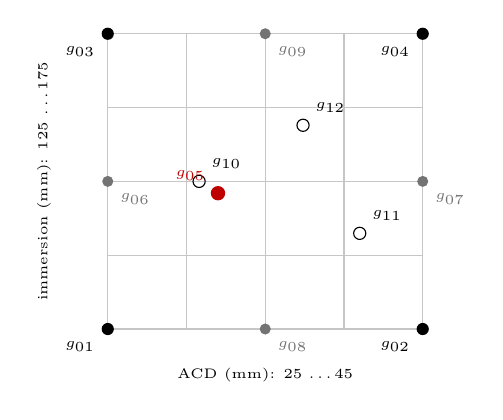
\begin{tikzpicture}[x=0.20cm,y=0.075cm]
  \draw[gray!45] (25,125) rectangle (45,175);
  \foreach \x in {25,30,35,40,45} \draw[gray!45] (\x,125)--(\x,175);
  \foreach \y in {125,137.5,150,162.5,175} \draw[gray!45] (25,\y)--(45,\y);
  \foreach \x/\y/\n in {25/125/01, 45/125/02, 25/175/03, 45/175/04}
     \fill[black] (\x,\y) circle (2.2pt) node[below left=1pt,font=\tiny] {$g_{\n}$};
  \foreach \x/\y/\n in {25/150/06, 45/150/07, 35/125/08, 35/175/09}
     \fill[black!55] (\x,\y) circle (2.0pt) node[below right=1pt,font=\tiny] {$g_{\n}$};
  \foreach \x/\y/\n in {30.8/150/10, 41/141.2/11, 37.4/159.5/12}
     \draw[black] (\x,\y) circle (2.2pt) node[above right=1pt,font=\tiny] {$g_{\n}$};
  \fill[red!75!black] (32,148) circle (2.6pt) node[above left=1pt,font=\tiny] {$g_{05}$};
  \node[font=\tiny,anchor=north] at (35,120) {ACD (mm): 25 \ldots 45};
  \node[font=\tiny,rotate=90,anchor=south] at (22,150) {immersion (mm): 125 \ldots 175};
\end{tikzpicture}
\end{center}

\noindent
Filled circles are corners, grey are edge midpoints, open are interior fills,
and $g_{05}$ in red is the nominal cell --- the geometry the existing campaign
was run at. Numerically:
\begin{center}
\small
\begin{tabular}{@{}lrrl@{}}
\toprule
& ACD & immersion & \\
\midrule
$g_{01}$ & $25.0$ & $125.0$ & corner \\
$g_{02}$ & $45.0$ & $125.0$ & corner \\
$g_{03}$ & $25.0$ & $175.0$ & corner \\
$g_{04}$ & $45.0$ & $175.0$ & corner \\
$g_{05}$ & $32.0$ & $148.0$ & \textbf{nominal} \\
$g_{06}$ & $25.0$ & $150.0$ & edge \\
$g_{07}$ & $45.0$ & $150.0$ & edge \\
$g_{08}$ & $35.0$ & $125.0$ & edge \\
$g_{09}$ & $35.0$ & $175.0$ & edge \\
$g_{10}$ & $30.8$ & $150.0$ & interior \\
$g_{11}$ & $41.0$ & $141.2$ & interior \\
$g_{12}$ & $37.4$ & $159.5$ & interior \\
\bottomrule
\end{tabular}
\end{center}
The corners are deliberate: they are where the geometry change is largest, so a
response that is low-rank there is low-rank everywhere between, and a design of
interior points alone could not establish that. Three points along each side is
the least that can distinguish curvature from a slope.

\paragraph{Where the box comes from}
It is a choice and not a derivation, and worth stating as such: a band about the
nominal cell, $-7/+13$~mm in gap and $-23/+27$~mm in immersion, wide enough that
a low-rank verdict means something and narrow enough to stay in a regime the
solver is known to handle. Three things bound it, none of which binds at these
values.

\emph{Resolution.} Chapter~1's mesh study finds that three nodes across the
anode--cathode gap ``is not a coarse approximation of a smooth field but a
failure to represent the layer at all''. The generator scales the layering with
the gap rather than holding the layer height fixed, so the gap carries
\emph{five} $z$-levels at every geometry in the box --- spacing $5.0$~mm at the
narrowest corner, $9.0$~mm at the widest --- and the small end is no less
resolved than the nominal cell. That constant layer count is also what makes the
relabelling of Section~\ref{sec:option0} possible, so the two facts are the same
fact.

\emph{Geometry.} The anode must remain partly clear of the bath. At $175$~mm the
box immerses under a third of a real anode ($584$~mm), so the constraint is not
approached.

\emph{Operation.} A reduction cell is run at a gap of a few centimetres, and the
box brackets that range rather than extrapolating beyond it.

What the box is \emph{not} is a validity domain for the surrogate. Nothing here
establishes that the response stays low-rank outside it, and the low-rank result
of this section is a statement about the interior of this rectangle only. Each
solve took between six and eight hours on eight cores, and the nominal geometry
$g_{05}$ reproduces the campaign's own mesh to the byte, which is the check that
the generator was driven correctly.

Two questions follow: whether the relabelling holds away from the two corners
already tested, and how many modes the geometry direction needs.

\paragraph{The relabelling is exact, at every point of the design box}
The twelve pilot geometries span the intended design --- anode--cathode distance
$25$ to $45$~mm, immersion $125$ to $175$~mm. Every one produces a mesh with the
same node and element counts as the campaign's own, and twelve different
numberings: hashing the connectivity and material arrays of five of them gives
five distinct pairs. Section~\ref{sec:option0} tested two corners; the
invariance holds over the whole box.

Applying the canonical order to all twelve, on both the velocity mesh and the
interface mesh, the connectivity after relabelling is \textbf{identical} every
time. The interface resolves into a single level, confirming that it is flat
before the free-surface loop runs, and its matched nodes are displaced
vertically by exactly zero --- the datum does not move, because the metal height
is held at its nominal value.

The displacements of the velocity mesh decompose as the geometry says they must,
which is the strongest evidence that the sort matches the right nodes. Every
vertical displacement is the design change itself, and the lateral motion
depends on the anode--cathode distance \emph{alone}: identical across the three
geometries sharing one value of it, and exactly zero across the three sharing
another. Its size is the wall cone applied to the vertical shift, in closed form
and agreeing to three figures.

This sharpens an earlier statement. The cone is indeed invariant under both
design parameters, but that does not make the \emph{nodes} laterally invariant:
a node sits at a fixed layer, the layer's height moves with the gap, and the
invariant cone is then sampled at a different height. Immersion does not enter
the layer heights and so moves nodes vertically only.

Each dump was also checked against its own solved mesh, where the two share a
numbering and differ only by the free-surface deformation. The discrepancies are
tens of millimetres, which is the interface excursion of
Section~\ref{sec:divergence} and nothing else --- metres would have meant the
two were not the same node list.

\label{meas:gate1}
\paragraph{The geometry direction is essentially one-dimensional}
Proper orthogonal decomposition of the twelve relabelled snapshots, mean
removed:
\begin{center}
\small
\begin{tabular}{@{}lrrrrrrr@{}}
\toprule
& \multicolumn{4}{c}{cumulative energy} & \multicolumn{3}{c}{modes needed} \\
\cmidrule(lr){2-5}\cmidrule(lr){6-8}
& 1 mode & 2 & 3 & 4 & $99\%$ & $99.9\%$ & $99.99\%$ \\
\midrule
velocity (\texttt{cuveb}) & $0.97898$ & $0.99248$ & $0.99880$ & $0.99962$ & 2 & 4 & 7 \\
interface $h$             & $0.98111$ & $0.99219$ & $0.99939$ & $0.99989$ & 2 & 3 & 5 \\
\bottomrule
\end{tabular}
\end{center}
Effective rank $1.04$ on both. A single mode carries $98\%$ of the response to a
$20$~mm change in ACD and a $50$~mm change in immersion together.

\label{rem:gate1-verdict}
\paragraph{Gate 1, read honestly}
The gate was fixed in advance: pass if three modes reach $99.9\%$, fail if eight
or more of the twelve are needed for $99\%$. Read against the table, the
interface passes as written and the velocity misses by six parts in ten
thousand. Both clear the failure criterion with two modes against a bar of
eight.

The gate should therefore be recorded as passed on its purpose and missed on its
letter, and the letter is the part to distrust. A threshold at $99.9\%$
discriminates between two numbers that differ in the third decimal, which twelve
snapshots cannot support. What the measurement establishes is what the gate
existed to ask: the geometry direction is low-dimensional, and interpolating in
it is safe.



\label{meas:geom-smooth}
\paragraph{Affine in geometry is enough for the velocity and not for the interface}
Low rank is necessary but not sufficient: Decision~2's pooled model writes
$\vect{A}(d,s) = \vect{A}_0 + \vect{A}_d\,\delta d + \vect{A}_s\,\delta s$, which
needs the modal coefficients to be \emph{affine} in $(d,s)$, not merely few.
With twelve design points a quadratic in $(d,s)$ has six parameters and six
residual degrees of freedom, so in-sample $R^2$ proves little; the column that
matters is the leave-one-out predictive $Q^2$.
\begin{center}
\small
\begin{tabular}{@{}lrrrrr@{}}
\toprule
& & \multicolumn{2}{c}{affine} & \multicolumn{2}{c}{$+$ quadratic} \\
\cmidrule(lr){3-4}\cmidrule(lr){5-6}
mode & evr & $R^2$ & $Q^2$ & $R^2$ & $Q^2$ \\
\midrule
\multicolumn{6}{@{}l}{\emph{velocity}} \\
1 & $0.97898$ & $0.9997$ & $0.9995$ & $1.0000$ & $1.0000$ \\
2 & $0.01350$ & $0.9790$ & $0.9491$ & $0.9983$ & $0.9845$ \\
3 & $0.00632$ & $0.0117$ & $-0.9875$ & $0.9934$ & $0.9749$ \\
4 & $0.00081$ & $0.0078$ & $-1.5434$ & $0.9816$ & $0.8483$ \\
\midrule
\multicolumn{6}{@{}l}{\emph{interface}} \\
1 & $0.98111$ & $0.9667$ & $0.9368$ & $0.9996$ & $0.9991$ \\
2 & $0.01108$ & $0.0455$ & $-0.9726$ & $0.9625$ & $0.7992$ \\
3 & $0.00720$ & $0.7052$ & $0.2335$ & $0.9789$ & $0.8602$ \\
4 & $0.00050$ & $0.2711$ & $-0.7035$ & $0.8807$ & $0.1627$ \\
\bottomrule
\end{tabular}
\end{center}
$Q^2$ tracks $R^2$ closely on the quadratic fits of the leading modes, so the
second order is real structure and not six parameters chasing twelve points.
Weighting each mode by its share of the field variance and counting only
out-of-sample skill:
\begin{center}
\small
\begin{tabular}{@{}lrr@{}}
\toprule
field variance predicted out of sample & affine in $(d,s)$ & quadratic in $(d,s)$ \\
\midrule
velocity  & $0.9913$ & $0.9991$ \\
interface & $0.9207$ & $0.9953$ \\
\bottomrule
\end{tabular}
\end{center}

\paragraph{Geometry is a far easier input than current}
Set beside the rest of this note, these numbers are remarkable. The response to
the $24$ currents needs $46$--$64$ modes and a network: a linear map of the
currents reaches $0.87$ of the field variance and the network $0.98$. The
response to the two geometry parameters needs \emph{one} mode for $98\%$, and a
six-term polynomial predicts $99.9\%$ of it on a geometry it has never seen.

The asymmetry is not surprising once stated --- moving an anode current
redistributes the forcing within a fixed domain, while moving the gap or the
bath level rescales the domain itself, which is a smoother thing to do --- but it
has a practical consequence for the campaign. The expensive direction to sample
is the current one, not the geometry one. A design that spends its runs on many
geometries and few current vectors per geometry is the wrong way round, which is
what the foldover of Section~\ref{sec:hadamard} already implies and what the
budget of that section assumes.

The caveat is the same one that runs through this section: every point here is
at \emph{uniform} current, so this measures $\vec g \mapsto \vec u(\vec g,
\vec I_{\mathrm{unif}})$ and not the way the current response itself changes with
geometry. The latter is what $\varrho$ of \eqref{eq:rho} is for, and it is
unmeasured.

\begin{corollary}[A correction to the campaign design]
\label{cor:geom-quadratic}
The affine expansion in $\vec g$ is adequate for the velocity, which it
reproduces to $99.1\%$ out of sample, and \emph{not} for the interface, where it
leaves $7.9\%$ of the variance unexplained --- an order of magnitude more than
the surrogate's own error. Since the operationally interesting objectives
(flatness, local ACD margin, short-circuit risk) are interface objectives, this
is exactly where it matters.

The remedy is cheap. Carrying $\{1, \delta d, \delta s, \delta d^2, \delta s^2,
\delta d\,\delta s\}$ instead of $\{1, \delta d, \delta s\}$ takes the pooled
model from $3\times(24+40) = 192$ to $6\times(24+40) = 384$ unknowns per mode,
so against the planned ${\approx}1\,800$ runs the oversampling falls from
$9.4\times$ to $4.7\times$ --- thinner, but still comfortable, and the design
must simply contain at least six distinct geometries, which the 24-point sweep
does many times over. Recording it now avoids discovering it after the campaign.
\end{corollary}

\label{meas:position-map}
\paragraph{The mesh itself is a closed-form function of the design}
The relabelled frame is a node-index frame: the surrogate predicts the field at
logical node $k$, and node $k$ is at a different place in every geometry --- up
to $70$~mm apart (Section~\ref{sec:gate1}). Placing a prediction in
physical space therefore appears to require that geometry's mesh, which is
sixteen minutes of meshing and would defeat a millisecond surrogate.

It does not. Fitting, per node and per component,
\[
  \vect{X}(d,s) \;=\; \vect{X}_0 + \vect{X}_d\,\delta d + \vect{X}_s\,\delta s
\]
over all $401\,838$ nodes and validating by leave-one-out over the twelve
geometries gives a worst-case node-position error of $13.2\ \mu$m and a median
of $11.0\ \mu$m. Elements are tens of millimetres, so this is $5\times10^{-4}$
of one element. Three arrays --- a base mesh and two derivatives --- reproduce
the mesh anywhere in the design box.

\begin{corollary}[The map $\varphi$, obtained rather than constructed]
\label{cor:phi-measured}
Chapter~2's conclusions call for a map $\varphi$ from a reference domain to the
physical domain, available in closed form, cheap and differentiable, and set out
to build one from the geometry. Section~\ref{sec:gate1} \emph{is}
that map, and it was not built: it is affine in $\vec g$, exact to $13\ \mu$m,
trivially differentiable, and it fell out of the relabelling as a by-product.
Its structure agrees with the geometry term by term ---
$\delta z = \delta d + \delta s$, lateral motion
$\delta d/\tan\alpha$ depending on ACD alone
(Section~\ref{sec:gate1}) --- so it is the analytic map, measured
rather than derived, with the layer bookkeeping done by the mesh generator
instead of by hand.

The deliverable of the geometry extension is therefore
\[
  (d,\,s,\,\vect{I}) \;\longmapsto\; \bigl(\text{field values at logical nodes},\
  \text{node positions}\bigr),
\]
both in milliseconds and with no call to the mesher. And the last reason to
prefer a fixed resampling grid --- that its output is a function on physical
space without further work --- is removed: so is the relabelled frame's.
\end{corollary}

\subsection{Incompressibility across geometries}
\label{sec:divergence}

Section~\ref{auto:corrections-to-the-transfer-construction} argued that a transfer between meshes cannot be expected to
preserve the discrete divergence, and proposed a Helmholtz--Hodge projection to
restore it. With the relabelling there is no transfer, but the objection does
not vanish with it: a POD mode is a linear combination of snapshots that each
satisfy a \emph{different} discrete divergence operator $\vect{B}_g$, because
$\vect{B}_g$ depends on node positions and those now differ by up to $70$~mm.
The question is what that costs, and it had never been measured.

\label{meas:eta-baseline}
\paragraph{The solver's own velocity is divergence-free to $3.4\%$}
For a $\mathbb{P}_1$ field on tetrahedra the gradient is exact and constant per
element, so
\[
  \eta \;=\; \frac{\|\nabla\cdot\vect{u}\|_{L^2(\Omega)}}
                  {\|\nabla\vect{u}\|_{L^2(\Omega)}}
\]
is an element sum with no quadrature error of its own. On the fluid submesh
($200\,925$ nodes, $1\,080\,960$ tetrahedra), over eight test runs of the
existing campaign, the median is
\[
  \eta_{\text{solver}} \;=\; 3.41\times10^{-2}.
\]
This is not a defect. The solver assembles SUPG together with a
Brezzi--Pitkäranta Laplace term on equal-order
$\mathbb{P}_1$--$\mathbb{P}_1$ \cite{hughes,brezzi-pitkaranta},
so the discrete velocity is never pointwise divergence-free; $3.4\%$ \emph{is}
the stabilisation level, and it is the benchmark any statement about
incompressibility here must be measured against. Evaluating a run's values on
the reference geometry's node positions instead of its own changes $\eta$ by
$0.0\%$ (ratio $1.00$ on all eight runs): within a geometry, interface motion of
a few millimetres contributes nothing.

\label{meas:eta-cross}
\paragraph{Stacking twelve geometries costs nothing}
The same quantity on the geometry pilot, where the nodes move by up to $70$~mm.
Evaluating $g_{01}$'s field on another geometry's mesh raises $\eta$ from
$3.22\times10^{-2}$ to $3.54$--$3.73\times10^{-2}$, a $10$--$16\%$ increase. And
for the reconstruction itself --- the object that actually matters, each
geometry's field rebuilt from the pooled basis and evaluated on the mesh it
claims to live on:
\begin{center}
\small
\begin{tabular}{@{}lrrr@{}}
\toprule
& $k=1$ & $k=3$ & $k=6$ \\
\midrule
median $\eta$, reconstruction & $3.395\times10^{-2}$ & $3.417\times10^{-2}$ & $3.420\times10^{-2}$ \\
median $\eta$, solver         & \multicolumn{3}{c}{$3.427\times10^{-2}$} \\
ratio                          & $0.99$ & $1.00$ & $1.00$ \\
\bottomrule
\end{tabular}
\end{center}
A reconstruction built from snapshots on twelve different meshes is as
divergence-free as the solver's own output, on every geometry and at every
truncation.

\begin{corollary}[The Helmholtz projection is withdrawn]
\label{cor:no-projection}
The projection was proposed as insurance; the insurance is not needed, and
taking it out would be a mistake rather than a missed refinement. Imposing
$\vect{B}_{\mathrm{ref}}\vect{u} = 0$ exactly would make the surrogate's output
\emph{more} divergence-free than the solver it is trained to reproduce --- a
discrepancy dressed as a guarantee. The mechanism is
Section~\ref{sec:divergence}: the stabilisation residual is an order of
magnitude larger than anything the mesh mismatch contributes, so there is no
room for the mismatch to matter.

This also settles \texttt{rem:ml-constraints} on firmer ground than it claimed
for itself. The thesis concedes that the linearity argument ``degrades with the
amplitude of the interface deformation''. It does not degrade, even at $70$~mm
of node motion, and the reason is that the operator being preserved is itself
only satisfied to $3.4\%$.

One caveat. These reconstructions use exact modal coefficients, not surrogate
predictions; a trained network contributes its own $2$--$3\%$ field error, which
carries its own divergence. That is the same order as the residual and so will
not dominate, but it should be measured again on predicted fields once the
$(d,s,\vect{I})$ surrogate exists.
\end{corollary}


\label{meas:dome}
\paragraph{Why a fixed resampling grid is not the alternative}
The natural alternative to relabelling is to resample every run onto one grid
fixed in physical space. For this cell that fails, and not marginally. The
metal--bath interface is not a slightly perturbed plane: over the
$11\,025$ nodes of the interface mesh it spans
\[
  z \in [0.0803,\ 0.1666]\ \text{m}, \qquad
  \text{span } 86.3\ \text{mm} = 2.7 \times \mathrm{ACD},
\]
against a datum $\texttt{geom\_z0} = 0.150$~m and a metal pad $150$~mm thick.
It is a dome: raised some $15$~mm in the interior and plunging to $70$~mm below
the datum at the perimeter, where it meets the sloped walls. The datum is the
mean level and not a bound --- the area-weighted mean height is $0.15007$~m,
within $0.07$~mm of $\texttt{geom\_z0}$, as volume conservation requires --- so a
grid plane there cuts the interface rather than bounding it, and puts
\textbf{$35.8\%$ of the interface area on the wrong side} ($22.61$ of
$63.21\ \mathrm{m^2}$; $4\,192$ of $11\,025$ nodes). Entry $k$ of the snapshot
vector would then be in liquid metal for one run and in electrolytic bath for
another. Since the
geometry moves the fluid column top while the datum stays fixed, which entries
change material is itself a function of $(d,s)$: the resampling would inject a
geometry-correlated artefact into precisely the matrix it is meant to clean.

The same objection applies at the other free surface. Under an anode the fluid
stops at $h + \mathrm{ACD}$, and grid points above it lie inside the anode; that
excluded set also moves with $(d,s)$.

A grid conforming to the interface would answer both --- build it in a layer
coordinate between the surfaces $z=0$, $z=h(x,y)$ and the local fluid top, so
that the interface is exactly a grid level --- but it buys nothing the
relabelling does not already give, at the price of a second interpolation error
on top of the discretisation error. It is recorded here as the fallback, not the
plan.

\label{rem:box-identity}
\paragraph{The resampling machinery works, and is the fallback}
The fallback was implemented and verified before being set aside, so that it is
available if the relabelling should fail on some future mesh family.
\texttt{post/create\_box3d.mac} builds a structured tetrahedral box by
\texttt{mesh/struct3d.mac} followed by \texttt{mesh/hexa\_tetra.mac}, the
three-dimensional counterpart of \texttt{post/create\_plane.mac}; and
\texttt{stat/perform\_postpro\_ref3d.mac} resamples \texttt{fluid\_vitesse} and
the level set \texttt{fluid\_phi} onto it by \texttt{data/interpolate.mac},
following \texttt{post/perform\_postpro\_midacd.mac}. On an identity test ---
interpolating a field whose value is the node coordinate itself onto a box
strictly inside the source mesh --- all $5\,551$ box points were located and the
maximum error was $9.99\times10^{-16}$, i.e.\ exact. The construction is sound;
it is the \emph{flat} choice of grid, not the interpolation, that
Section~\ref{sec:divergence} rules out.

\label{rem:two-materials}
\paragraph{Two materials, and what actually matters about them}
The fluid domain holds two fluids, and it is worth being precise about which of
their differences bear on the construction. Their densities differ,
$\rho_{\text{Al}} = 2270$ against $\rho_{\text{bath}} = 2130\ \mathrm{kg/m^3}$
(\texttt{veloc\_rho1}, \texttt{veloc\_rho2}), and the pressure space is
discontinuous across the interface (\texttt{ns3d\_cont\_press} $= 0$), which is
what lets the discretisation carry the jump in $\nabla p$ that balances the jump
in $\rho \vec g$. The viscosity, by contrast, is \emph{not} split by phase: the
tensor \texttt{fluid\_mu\_\#1..\#9} is assembled from
$\texttt{veloc\_mud}_{1,2,3}$ with no phase index, and the run log confirms a
single isotropic value $2\times10^{-3}$ throughout. So the velocity is
continuous with continuous gradient across the interface, and the smoothness
argument one might expect to make against a non-conforming grid does not apply.

What does apply is Section~\ref{sec:divergence}, and it is geometric rather than
analytic: the objection to a fixed grid is not that the solution is rough at the
interface but that the interface is $86$~mm from flat, so a fixed grid cannot
keep a given entry on one side of it across runs. The relabelling is immune
because it never asks where a node is --- only which logical node it is --- and
the material partition travels with the node.

\iffalse
\label{cor:transfer-required}
\paragraph{The transfer construction is required}
Changing the anode--cathode distance produces a mesh with the same
combinatorial size and the same material partition but a different numbering.
Snapshots at different geometries therefore cannot be stacked into
$\vect{G}$ as they stand, and the reference-domain construction of
Chapter~2's conclusions --- a fixed reference mesh, the map $\varphi$, a
transfer operator and a projection restoring the discrete constraint --- is
necessary rather than optional. Proposition~\ref{prop:piola} and
Section~\ref{auto:corrections-to-the-transfer-construction} are therefore load-bearing, not hypothetical: the
pull-back must be the one written there, and the divergence guarantee must be
re-established by Helmholtz projection because interpolation will not preserve
it.
\fi

\label{rem:opt0-residual}
\paragraph{What the invariant counts still buy}
The negative result is not without consequence for the design. Because the
element count, the node count and the material partition are \emph{exactly}
preserved, the two meshes are of the same size and resolution, and the
difficulty is a relabelling rather than a genuinely different discretisation.
A transfer between them is therefore an interpolation between two meshes of
equal fineness --- the benign case for
Section~\ref{auto:corrections-to-the-transfer-construction}(b) --- and the reference mesh of Phase~1 can be taken to
be the mesh of any one geometry rather than a specially refined one. It also
means the round-trip test of Phase~1 has a natural null hypothesis: at
identical geometry the transfer must be the identity to machine precision.

\subsection{Does the transfer reduce the rank? A free pilot says no}
\label{sec:transfer-pilot}

Chapter~2's conclusions expect the reference-domain transfer to \emph{improve}
the decomposition, on the grounds that the node-index frame ``conflates a change
of the field with a change of the mesh''. That expectation is testable without
any solver run, because the existing campaign already has a fluid domain whose
shape varies: the mesh follows the deformed interface, so node $k$ sits in a
slightly different place in every run.

\label{def:transfer}
\paragraph{First-order transfer}
All runs share connectivity and node identity, and the displacement is a few
millimetres against a mesh size of tens of millimetres, so the pull-back to the
reference positions is
\begin{equation}
\label{eq:taylor-transfer}
\vec{u}_i^{\mathrm{ref}}(\vect{X}_{\mathrm{ref}})
= \vec{u}_i(\vect{X}_i)
+ (\nabla\vec{u}_i)\cdot(\vect{X}_{\mathrm{ref}}-\vect{X}_i)
+ O(|\delta\vect{X}|^2),
\end{equation}
with the gradient exact per tetrahedron for a $\mathbb{P}_1$ field and averaged
to nodes with volume weights. This is not yet the Piola transform: at this stage
the map is a small displacement of the \emph{same} mesh, so the Jacobian is the
identity to the order retained. The Piola question arises only where the
geometry genuinely differs.

\label{meas:motion-share}
\paragraph{How much of a snapshot is mesh motion}
Over twelve randomly drawn training runs, the correction term of
\eqref{eq:taylor-transfer} has norm $0.10$ to $0.38$ of the learned perturbation
$\|\vec{u}_i-\vec{u}_{\mathrm{ref}}\|$, median $0.14$. The largest values
coincide with the largest displacements, up to $65$~mm on a strongly deformed
run. So the transfer would move about a seventh of a typical snapshot ---
enough to matter, not enough to dominate.

\label{meas:pilot}
\paragraph{The transfer does not reduce the rank; it slightly increases it}
All $1\,194$ training runs were transferred by \eqref{eq:taylor-transfer} and the
decomposition recomputed, $\Delta$ about the reference run, in both frames:
\begin{center}
\small
\begin{tabular}{@{}lrrrrr@{}}
\toprule
frame & eff.\ rank & $n_{90}$ & $n_{95}$ & $n_{99}$ & top 3 \\
\multicolumn{6}{@{}l}{\footnotesize $n_q$ = modes needed for a fraction $q$ of the variance}\\
\midrule
node-index (as deployed) & $13.48$ & $19$ & $24$ & $46$ & $37.6\%$ \\
reference (transferred)  & $13.98$ & $19$ & $25$ & $49$ & $36.7\%$ \\
\bottomrule
\end{tabular}
\end{center}
The node-index row reproduces Chapter~2 exactly (effective rank $13.5$,
$n_{99} = 46$), which validates the decomposition against the published figures.
The transferred row is marginally \emph{worse} on every criterion. The
expectation that the rank would fall from $46$ to about $30$ is not met.

\label{rem:pilot-why}
\paragraph{Why, and why it is not a bug}
The round-trip check confirms the implementation: transferring a run to the
reference frame and back reproduces it to a relative $L^2$ of
$3.7\times10^{-4}$ to $1.1\times10^{-3}$, and \emph{exactly} zero for the
reference run itself, where $\delta\vect{X} = 0$. The negative result is
therefore about the data and not about the code.

The explanation is that the mesh motion is not an independent contamination. The
mesh follows the interface, the interface is driven by the anode currents, and
the flow is driven by the same currents --- so the apparent ``mesh'' variation
lies in the same low-dimensional response as the field variation it is supposed
to be polluting. Removing it does not simplify the solution manifold, and the
first-order reconstruction adds a little gradient noise of its own.

\label{cor:transfer-purpose}
\paragraph{What the transfer is for}
This result is what makes Corollary~\ref{cor:relabel-not-transfer} possible.
Had the transfer reduced the rank, it would have been worth its interpolation
error even once the relabelling removed the obligation to use it; it does not,
so nothing is lost by dispensing with it. The two findings are independent --- one
says the correspondence can be recovered by sorting, the other that recovering
it in a common physical frame buys nothing --- and only together do they close
the question.

One consequence for the next phase. The mode count for the geometry campaign
should be planned at the $k$ the present field already needs, of order
$46$--$64$, and not at the $\approx30$ the earlier reasoning suggested: no
reduction is coming from the change of frame, because there is no change of
frame.

\subsection{Corrections to the transfer construction}
\label{auto:corrections-to-the-transfer-construction}

The transform below is the contravariant Piola map, standard for
$H(\mathrm{div})$-conforming spaces \cite{bbf}; the point of stating it is that
the direction matters and the thesis has it reversed.

\begin{proposition}[The Piola pull-back]
\label{prop:piola}
Let $\varphi:\hat{D}\to D$ with $\vect{J} = \nabla\varphi$. The contravariant
Piola transform pushes a reference field forward by
$\vec{u} = \det(\vect{J})^{-1}\vect{J}\,\hat{\vec{u}}$; consequently the
pull-back of a physical field to the reference domain is
\begin{equation}
\label{eq:piola}
\hat{\vec{u}} \;=\; \det(\vect{J})\,\vect{J}^{-1}\,(\vec{u}\circ\varphi),
\end{equation}
and not $\det(\vect{J})^{-1}\vect{J}(\vec{u}\circ\varphi)$, which is the
push-forward applied in the wrong direction.
\end{proposition}

\label{rem:div}
\paragraph{The divergence-free guarantee and its three failure modes}
Discrete incompressibility is a \emph{linear} constraint
$\vect{B}\vec{u} = \vec{0}$. If a single operator $\vect{B}$ is shared by all
snapshots, then every mode --- being a linear combination of centred snapshots
--- lies in $\ker\vect{B}$, and so does every reconstruction
\eqref{eq:surrogate}. The guarantee fails for three independent reasons.
\emph{(a)} $\vect{B}$ depends on node positions, which differ between runs
because the mesh follows the interface; the guarantee is exact only for a fixed
mesh. \emph{(b)} Nodal interpolation between non-nested meshes is $O(h^2)$ in
$L^2$ but only $O(h)$ in $H^1$; since $\dive$ is a first derivative and
$\dive\vec{u}_h$ is itself a small stabilisation residual, the interpolation
error is $O(1)$ \emph{relative to the quantity being preserved}, and the Piola
transform, being a change of variables rather than a gradient-controlling
projection, does not repair this. \emph{(c)} With stabilised equal-order
elements the solver's own velocity is not pointwise divergence-free: it satisfies
$\int q\,\dive\vec{u}_h = 0$ over the pressure space at best. The target is
therefore the solver's stabilisation level and not zero.

All three are correct as statements about interpolation between different
discretisations, which is why they remain on record. None of them bites on the
construction actually adopted. Section~\ref{sec:divergence} measures that level
--- $3.4\times10^{-2}$, an order of magnitude above the initial estimate made
here --- and finds that a decomposition pooled over twelve differently numbered
meshes reaches it exactly. The Helmholtz--Hodge projection proposed as insurance
against \emph{(a)} is therefore withdrawn
(Section~\ref{sec:divergence}); \emph{(b)} does not arise because nothing is
interpolated; and \emph{(c)}, once measured rather than estimated, turns out to
dominate the other two by so much that neither can be detected.

\subsection{Orthogonal designs for estimating $\vect{A}$}
\label{sec:hadamard}

The design below is a foldover on the rows of a Hadamard matrix, constructed by
the Paley method \cite{hedayat}; foldover and its aliasing properties are
standard \cite{bhh}, and the conditioning it buys is what $D$-optimality
maximises \cite{atkinson}.

\begin{proposition}[Hadamard design]
\label{prop:hadamard}
Since $23$ is prime, the Paley construction gives a Hadamard matrix
$\vect{H}$ of order $24$. Let $\vect{R} \in \{\pm1\}^{23\times24}$ consist of
its rows $2,\dots,24$ in normalised form. Then
\begin{enumerate}
\item each row of $\vect{R}$ contains exactly twelve $+1$ and twelve $-1$, hence
$\vect{R}\vec{1} = \vec{0}$, so the constraint $\sum_j p_j = 0$
holds \emph{by construction};
\item $\vect{R}\vect{R}^{\mathsf{T}} = 24\,\vect{I}_{23}$, so the rows are
mutually orthogonal and span the constraint hyperplane;
\item scaling by
$A^{*} = \min(I_{\mathrm{mean}}-I_{\min},\,I_{\max}-I_{\mathrm{mean}}) = 3\,983$~A
is the largest symmetric amplitude that keeps every anode feasible, and it
saturates the upper bound exactly.
\end{enumerate}
\textnormal{All three verified numerically: the Gram matrix has diagonal $24$
and off-diagonal exactly $0$, and the resulting current vectors satisfy
$\sum_j I_j = 490\,000$~A with $\max = 24\,400$~A on the bound and
$\min = 16\,434$~A, some $34$~A above it. The box is asymmetric about the mean
--- $4\,017$~A of room below against $3\,983$~A above --- so a symmetric design
cannot reach both bounds at once, and the binding side is the upper one.}
\end{proposition}

\begin{lemma}[Foldover separates odd and even orders exactly]
\label{lem:foldover}
Let $\vec{c}(\vec\delta)$ be any map admitting the expansion
$\vec{c}(\vec\delta) = \vec{c}_0 + \vect{A}\vec\delta + \vect{Q}(\vec\delta,\vec\delta)
+ O(\|\vec\delta\|^3)$ with $\vect{Q}$ bilinear symmetric. Then
\begin{equation}
\label{eq:foldover}
\tfrac12\bigl(\vec{c}(\vec\delta)-\vec{c}(-\vec\delta)\bigr)
= \vect{A}\vec\delta + O(\|\vec\delta\|^3),
\qquad
\tfrac12\bigl(\vec{c}(\vec\delta)+\vec{c}(-\vec\delta)\bigr) - \vec{c}_0
= \vect{Q}(\vec\delta,\vec\delta) + O(\|\vec\delta\|^4).
\end{equation}
Hence running each design row at $+\vec\delta$ and $-\vec\delta$ makes the
estimate of $\vect{A}$ unbiased under \emph{arbitrary} even-order nonlinearity,
and yields the quadratic form along that direction at no additional cost. The
scalar
\begin{equation}
\label{eq:rho}
\varrho \;=\;
\frac{\bigl\|\tfrac12(\vec{c}(\vec\delta)+\vec{c}(-\vec\delta))-\vec{c}_0\bigr\|}
     {\bigl\|\tfrac12(\vec{c}(\vec\delta)-\vec{c}(-\vec\delta))\bigr\|}
\end{equation}
is therefore an exact measure of the ratio of quadratic to linear response, and
is a cleaner nonlinearity probe than a difference of ridge-regularised fits.
\end{lemma}

\begin{proof}
Substitute $-\vec\delta$ and use $\vect{A}(-\vec\delta) = -\vect{A}\vec\delta$
and $\vect{Q}(-\vec\delta,-\vec\delta) = \vect{Q}(\vec\delta,\vec\delta)$; odd
terms cancel in the sum and even terms in the difference.
\end{proof}

\paragraph{Sample efficiency, and what it costs}
Under random Gaussian $\vec\delta$ the expected out-of-sample $R^2$ of
$\vect{A}$ with $p=23$ predictors and $N$ runs is
$1-\sigma^2/\mathrm{Var}\cdot(1+(p+1)/(N-p-2))$, which with the measured
$\sigma^2/\mathrm{Var} = 0.185$ is \emph{negative} at $N=30$ and reaches only
$\approx0.73$ at $N=75$. The $46$-run foldover design carries the information of
$230$--$250$ random runs. Note that Lemma~\ref{lem:foldover} leaves a cubic bias
at full box amplitude; running both $\pm4$ and $\pm2$~kA and taking
$\vect{A}_0 = (4\vect{A}_2-\vect{A}_4)/3$ removes it to leading order.

\label{rem:counting}
\paragraph{Parameter counting for a pooled model}
Per modal coefficient, $\vect{A}$ has $24$ unknowns and a full quadratic form
$\vect{Q}$ has $\binom{24}{2}+24 = 300$, so $324$ in total. Fitting each
geometry independently at fivefold oversampling costs $\approx1\,620$ runs per
geometry; for $24$ geometries, $\approx38\,900$ runs. Positing instead that the
coefficients vary affinely in a two-dimensional geometry parameter
$\vec{g}=(d,s)$,
\begin{equation}
\label{eq:pooled}
\vec{c}(\vec{g},\vec\delta) = \vect{A}(\vec{g})\,\vec\delta
+ \vect{Q}(\vec{g})(\vec\delta,\vec\delta)+\dots,
\qquad
\vect{A}(\vec{g}) = \vect{A}_0 + \vect{A}_d\,\delta d + \vect{A}_s\,\delta s,
\end{equation}
gives $3\times324 = 972$ unknowns per mode for the \emph{entire} campaign. With
the screening of Definition~\ref{def:predictors} retaining $40$ products this is
$3\times(24+40) = 192$ per mode, i.e.\ about ninefold oversampling against a
budget of $\approx1\,800$ runs.

Two corrections to that count, both from measurements made after it was written.
The affine dependence on $\vec{g}$ assumed in \eqref{eq:pooled} is
\emph{not} adequate for the interface
(Corollary~\ref{cor:geom-quadratic}): carrying the three second-order geometry
terms as well doubles the count to $384$ per mode and reduces the oversampling
to $4.7\times$, which is the figure to budget against. And the counts $24$ and
$300$ are the sizes of the design blocks, not of the identifiable parameter
sets: by Proposition~\ref{prop:rank} only $23$ directions are ever exercised, so
the true counts are $23$ and $276$. Using the larger numbers makes the
oversampling estimate conservative, which is the safe direction for a budget.

What remains untested is the premise itself --- that $\vect{A}$ and $\vect{Q}$
vary smoothly in $\vec{g}$ at all. Section~\ref{sec:gate1} measures the geometry
response at uniform current and finds it low-dimensional, but that is the
response and not the \emph{map}; establishing the latter needs current
perturbations at several geometries, and \eqref{eq:rho} is the instrument.

\subsection{What the campaign costs, and what fits}
\label{sec:cost}

The design of Section~\ref{sec:hadamard} is affordable only against a stated
budget, and the numbers below are measured rather than estimated: the scheduler
prices a production-sized job --- eight tasks, eight hours, which is what the
twelve pilot solves actually took --- at \textbf{CHF~$0.35$}, and the twelve
consumed $57.4$ core-hours each.

A sweep geometry is $46$ foldover runs, one base run at uniform current and
seven interior points, so $54$; an anchor geometry runs the foldover at two
amplitudes to cancel the cubic bias of Lemma~\ref{lem:foldover}, so $93$. Adding
the $\varrho$ gate and one held-out geometry:

\begin{center}
\small
\begin{tabular}{@{}lrrr@{}}
\toprule
configuration & runs & CHF & against the allocation \\
\midrule
$24$ sweep, $2$ anchors, $\varrho$ on a cross of five & $1\,837$ & $643$ & $-177$ \\
$24$ sweep, $2$ anchors, $\varrho$ on three points    & $1\,752$ & $613$ & $-147$ \\
$20$ sweep, $2$ anchors, $\varrho$ on a cross         & $1\,621$ & $567$ & $-101$ \\
$16$ sweep, $2$ anchors, $\varrho$ on a cross         & $1\,405$ & $492$ & $-25$ \\
$16$ sweep, $2$ anchors, $\varrho$ on three points    & $1\,320$ & $462$ & $+4$ \\
$16$ sweep, $1$ anchor,  $\varrho$ on three points    & $1\,227$ & $429$ & $+37$ \\
\midrule
\textbf{the $\varrho$ gate alone, on a cross of five} & $235$ & $82$ & $+384$ \\
the $\varrho$ gate alone, on three points             & $150$ & $53$ & $+414$ \\
\bottomrule
\end{tabular}
\end{center}

\noindent
The allocation is a cap of CHF~$1\,000$ on the account, of which CHF~$534$ is
already consumed, leaving \textbf{CHF~$466$} at the time of writing. The
campaign as designed does not fit, and the two configurations that do fit spend
the entire remainder, leaving nothing for a re-run, a failed job, or any other
work on the account for the rest of the period.

\paragraph{What shrinking the sweep costs}
Not identifiability --- the pooled design remains full rank down to $16$ sweep
geometries --- but conditioning. Building the design matrix for the quadratic
geometry model of Corollary~\ref{cor:geom-quadratic} and taking its singular
values:
\begin{center}
\small
\begin{tabular}{@{}lrrl@{}}
\toprule
sweep geometries & oversampling & condition number & \\
\midrule
$24$ & $3.9\times$ & $438$ & \\
$20$ & $3.3\times$ & $639$ & \\
$16$ & $2.8\times$ & $2\,703$ & \\
$14$ & $2.5\times$ & --- & \textbf{rank deficient} \\
\bottomrule
\end{tabular}
\end{center}
The degradation is not gradual. Going from $24$ to $20$ costs a factor $1.5$ in
conditioning; from $20$ to $16$ costs a factor $4.2$; and at $14$, or at $16$
with the interior points cut from seven to five, the design stops being
identifiable at all rather than becoming gradually worse. The cliff sits
immediately below where the budget forces the design.

\paragraph{Recommendation}
Run the $\varrho$ gate first and decide afterwards. It costs CHF~$82$, under a
fifth of what remains, and it answers the question on which the other CHF~$535$
depends --- whether $\vect{A}$ varies smoothly enough in $\vec g$ for the pooled
model to be legitimate at all. It also measures the one quantity the budget
silently assumes and nothing has checked: the convergence rate at the corners of
the design box under a full-amplitude current perturbation. Every pilot run
converged, but every pilot run was at uniform current; if corner acceptance is
$80\%$ rather than the $\approx100\%$ the nominal-geometry campaign enjoyed,
every figure in the table above is optimistic by a quarter.

If the gate passes, the honest options are to raise the cap or to accept
$16$ sweep geometries at a conditioning of $2\,700$ and no contingency. Of the
two, raising the cap is the better engineering: CHF~$643$ against a cap of
CHF~$1\,000$ already half consumed is not an unreasonable request, whereas the
alternative spends everything on a design sitting one step above rank
deficiency.

\paragraph{Storage}
Not a constraint. The campaign master and per-run exports run to about
$1.1$~GB per run, so $1\,800$ runs is some $2$~TB on top of the existing
$1.9$~TB. The filesystem has over a petabyte free and no project quota is
enforced.

% =====================================================================
\section{Summary of what is established and what is not}
\label{auto:summary-of-what-is-established-and-what}

Four statements carry the rest, and they are easier to hold together than the
list below.

\emph{First}, the network is needed for prediction --- of the velocity and the
interface, not universally. It beats a linear map in every sampled regime and by
the widest margin when the cell is least ordinary, which is when a model is most
wanted. But on the metal current density a \emph{linear} field model scores
$1.000$ and beats it, because there the linear residual is two parts in a
thousand rather than one part in eight. What decides the matter is the residual,
not the model class.

\emph{Second}, the quantities an engineer reads should be computed from a
predicted field and never regressed on the currents directly. Direct regression
is worse than predicting the mean on every velocity functional. This too is
governed by the residual, and it is subject to the same bound as everything
else: it holds inside the sampled regimes and fails outside them.

\emph{Third}, the network should \emph{not} be the thing an optimiser sees. With
the affine field model every objective considered here is strictly convex with a
unique optimum reached from every start; the irreproducibility measured on the
network is its own artefact. The flexibility that makes it the better predictor
is what makes it the worse objective, because where the data does not constrain
the map the network is free, and that freedom appears downstream as structure
that is not in the physics.

\emph{Fourth}, the campaign's coverage of rare operating conditions is
load-bearing and its regime mix is not an imbalance to be corrected. Removing a
condition from training breaks every model class equally.

\paragraph{Established, on existing data, with no new solver runs.}
\begin{itemize}\itemsep2pt
\item Functionals of a \emph{network}-predicted field beat direct regression on
every $L^1/L^2$ target ($0.97$--$0.99$ against $0.80$--$0.94$), and rescue the
cases where direct regression collapses to $R^2<0$; a \emph{linear}-predicted
field does not (Table~\ref{tab:main}). The implementation agrees exactly with
the solver on every $L^\infty$ functional (Section~\ref{sec:results}).
\item The residual of the best predictor is regression error, not basis error:
the truncation floor is $\approx1.000$ on every $L^1/L^2$ target
(Table~\ref{tab:floor}).
\item The metal current density has effective rank $5.9$ and is affine in the
currents to $R^2 = 0.9982$; the metal-pad-instability proxy built from it is
recovered at $R^2 = 1.000$ by a \emph{linear} field model and at $-0.107$ by
direct linear regression, so its nonlinearity is a property of the observable
and not of the cell (Proposition~\ref{prop:manufactured}).
\item Across $30$ functionals spanning five planes, three fields and three
continuity classes, predictor~(iv) is best on $28$; and the behaviour is
predicted by the functional's class rather than measured case by case ---
affine observables gain nothing from a field model
(Proposition~\ref{prop:affine}, confirmed to $0.009$), absolute observables are
recovered by a linear one, quadratic observables require an accurate one
(Corollary~\ref{cor:classification}).
\item Direct regression of an observable is not merely worse than evaluating it
on a predicted field --- on a cell with an anode being replaced it is
\emph{negative} where the field route returns $0.78$, while in ordinary
operation the two are within three percent of each other. The advantage is
concentrated in the conditions a model is actually consulted for
(Section~\ref{sec:per-regime}).
\item The network is better than a linear map in every regime the campaign
samples, by factors of two to fourteen, and its margin is largest where the cell
is least ordinary --- $2.4\%$ against $11.8\%$ during an anode replacement.
Remove a regime from training and no predictor of any class beats the mean on
it, so the result bounds what a campaign must \emph{cover} rather than which
model to use (Section~\ref{sec:boundary}).
\item $n \approx 400$--$600$ runs suffice for the linear operator at a fixed
geometry; the screened quadratic map has a stability threshold near $n=600$
rather than a smooth curve (Measurements~\ref{sec:curves},
\ref{sec:curves}).
\item $\rank\vect{A} = 23$ exactly, its spectrum is computable from a
$64\times24$ matrix (Lemma~\ref{lem:spectrum}), and its conditioning predicts
the reproducibility of the inverse design problem measured independently by
multi-start optimisation. That irreproducibility belongs to the surrogate and
not to the cell: with the affine field model every objective used here is
strictly convex and has a unique optimum, reached from every start
(Proposition~\ref{prop:convex}). The corollary for inverse design is to optimise
the convex model inside a trust region and let the network place the region
(Section~\ref{sec:inverse}).
\end{itemize}

\paragraph{Refuted, having been measured.}
\begin{itemize}\itemsep2pt
\item That a \emph{linear} field model suffices for functionals: column~(iii) of
Table~\ref{tab:main} scores $0.03$--$0.73$ and loses to direct quadratic
regression almost everywhere.
\item That retraining at the predictability truncation $k\approx24/24/7$
improves the surrogate: the total error against the full-resolution field
approximately doubles on all three targets, because the truncation error grows
faster than the regression error falls (Section~\ref{auto:retraining-at-the-predictability-truncat}). The
opposite conclusion follows from the existing tooling only because it
re-truncates the reference field with the model
(Section~\ref{auto:retraining-at-the-predictability-truncat}).
\item That the predicted interface violates volume conservation appreciably: it
violates it by $0.6$ times the solver's own residual, and imposing the
projection changes the error by $+0.01\%$ (Section~\ref{auto:imposing-volume-conservation-on-the-inte}).
\item That varying the anode--cathode distance within the constant-ACD regime
reintroduces the interface--gap--current feedback: that regime preserves the gap
pointwise at \emph{every} design ACD, so the feedback belongs to the
fixed-anode regime alone.
\item That immersion depth is uniquely problematic for a layer map: the wall cone
$\texttt{geom\_xb}(z) = W_x + z/\tan\alpha_x$ is invariant under both geometry
parameters, the ACD dependence cancelling identically.
\end{itemize}

\paragraph{Also refuted, by Tier~C.}
That the horizontal current in the metal is evidence for a nonlinear surrogate
(Section~\ref{sec:tierC}). And a latent defect found in passing:
\texttt{normalize: false} in the deployed configurations is calibrated to
velocity-scale coefficients and fails silently on a field with different units
(Section~\ref{sec:tierC}).

\paragraph{Established for the geometry extension.}
\begin{itemize}\itemsep2pt
\item The mesh generator does \emph{not} preserve node numbering under a change
of $(d,s)$, but it does preserve everything else: over the whole design box the
twelve pilot geometries give the same $401\,838$ nodes and $2\,109\,072$
elements with twelve different numberings
(Measurements~\ref{sec:option0}, \ref{sec:relabel-solved}). Ordering by
$(\text{level rank}, y, x)$ recovers the correspondence exactly, so snapshots at
different geometries are stacked by \textbf{relabelling}, with no reference
mesh, no map $\varphi$, no Piola pull-back and no interpolation
(Corollary~\ref{cor:relabel-not-transfer}).
\item The relabelling must be computed from the mesh as generated, not from the
solved mesh, whose level structure the free-surface loop destroys; the dump that
makes this possible costs about ten minutes per geometry and requires no run to
be repeated (Section~\ref{sec:relabel-solved}).
\item Carried out at all twelve pilot geometries, on both the velocity mesh and
the interface mesh, the relabelling gives \textbf{identical connectivity} every
time, and the matched-node displacements are the design changes in closed form:
$\delta z$ is $\delta d + \delta s$ exactly, and the lateral motion is the cone
law $\delta d/\tan\alpha$ to three figures, depending on ACD alone
(Section~\ref{sec:gate1}).
\item \textbf{The geometry direction is essentially one-dimensional}: one mode
carries $97.9\%$ of the velocity response and $98.1\%$ of the interface response
over the whole design box, effective rank $1.04$, two modes reach $99.2\%$
(Section~\ref{sec:gate1}). Gate~1 passes on its purpose; the velocity misses
its written threshold in the third decimal place, which is not a distinction
twelve snapshots can support (Section~\ref{sec:gate1}).
\item But \emph{affine} in $(d,s)$ is enough only for the velocity. Measured by
leave-one-out, the affine expansion predicts $99.1\%$ of the velocity variance
out of sample and only $92.1\%$ of the interface variance; adding the three
second-order geometry terms gives $99.9\%$ and $99.5\%$
(Section~\ref{sec:gate1}). Decision~2's pooled
$\vect{A}(d,s)$ therefore needs a quadratic in $\vec g$, at $4.7\times$ rather
than $9.4\times$ oversampling (Corollary~\ref{cor:geom-quadratic}).
\item Incompressibility survives the stacking untouched. The solver's own
velocity is divergence-free only to $\eta = 3.41\times10^{-2}$ --- SUPG plus a
Brezzi--Pitkäranta term on equal-order $\mathbb{P}_1$--$\mathbb{P}_1$ --- and a
POD reconstruction pooled over twelve different meshes reaches the same
$3.42\times10^{-2}$ at every truncation (Measurements~\ref{sec:divergence},
\ref{sec:divergence}). The Helmholtz projection proposed as insurance is
therefore \textbf{withdrawn}: it would make the surrogate more divergence-free
than the solver it reproduces (Corollary~\ref{cor:no-projection}).
\item The mesh itself is predictable: $\vect{X}(d,s)$ is affine to $13\ \mu$m
worst case by leave-one-out over all $401\,838$ nodes, so the surrogate returns
field values \emph{and} node positions in milliseconds with no call to the
mesher --- and this is the closed-form $\varphi$ Chapter~2 set out to construct
(Section~\ref{sec:gate1}, Corollary~\ref{cor:phi-measured}).
\item The alternative --- one grid fixed in physical space --- is ruled out for
this cell, and geometrically rather than analytically: the interface spans
$86$~mm, $2.7$ times the ACD, so a plane at the datum would put $35.8\%$ of the
interface area on the wrong side of it, and which entries change material is itself a
function of $(d,s)$ (Section~\ref{sec:divergence},
Section~\ref{sec:divergence}). The resampling machinery was nevertheless
implemented and verified to machine precision, and is kept as the fallback
(Section~\ref{sec:divergence}).
\end{itemize}

\paragraph{Established by composing the two surrogates.}
\begin{itemize}\itemsep2pt
\item Substituting the network's flow for the solver's changes the published
alumina homogeneity metric by $0.25\%$, against a velocity error of $0.59\%$:
the transport attenuates surrogate error rather than amplifying it
(Section~\ref{sec:composed-measured}).
\item Across operating conditions the same metric moves by $-14\%$ to $+7\%$ and
the alumina field by up to $9.7\%$ --- ten to forty times what predicting the
flow costs, so the effect is comfortably resolved. It is not monotone in the size
of the current disturbance, and the only condition that lowers the minimum
concentration is an anode being replaced.
\item A synthetic perturbation of the flow, used before the real residual was
available, over-estimated the sensitivity by a factor of thirty. Proxy
perturbations are not substitutes for measured residuals.
\end{itemize}

\paragraph{Not yet established.}
The functionals built from $\texttt{fields\_full/\{forces,induction\}}$, which
Chapter~2 measures to have coefficients of variation of $0.30\%$ and $0.22\%$
and which are therefore nearly invariant across the campaign. And everything that requires
currents and geometry to vary \emph{together}: the twelve pilot runs are all at
uniform current, so they measure the geometry response alone. Whether
$\vect{A}$ itself varies smoothly across the design box --- the nonlinearity
ratio $\rho$ of the plan's step~1.2 --- needs the current perturbations at
several geometries and is the next measurement, not this one.

% =====================================================================
\section{The question this opens}
\label{sec:opens}

Everything above treats the surrogate as the end of the pipeline. It is not. A
velocity field is an intermediate, and Section~\ref{sec:functionals} is really
the first case of a more general question: what happens when a predicted field
is handed to something downstream. There the something was a functional. In
practice it is another solver.

\paragraph{The chain, and who has surrogated which link}
Alumina is injected by a number of feeders, transported by the flow, dissolved,
and consumed at the anodes; local deficits cause anode effects and local
surpluses cause sludge, so its homogeneity is an operational target. The chain
is
\[
  \text{anode currents} \;\longrightarrow\;
  \text{MHD flow} \;\longrightarrow\;
  \text{dissolved alumina} .
\]
Patouillet et al.\ \cite{patouillet} surrogate the second link with the same
solver used here: a graph neural network maps seven feeder mass-flow fractions,
under a conservation constraint, to the dissolved-alumina field on the mid-ACD
plane, trained on some fifteen percent of $1\,443$ admissible combinations and
predicting in about a second. This note surrogates the first link. The two
studies hold still precisely what the other moves --- their currents are assumed
uniform across the anodes, and the feeders here are fixed --- so between them the
chain is covered exactly once, with no overlap and no composition.

\paragraph{The question}
\emph{Given a chain of physical models, where should the surrogate boundary be
drawn, and can the answer be predicted rather than discovered?} Three
configurations are available and they are not obviously ranked:
\begin{enumerate}
\item \textbf{end to end}: learn $(\text{currents},\text{feeders}) \mapsto
\text{alumina} $ as one map, so the flow never appears;
\item \textbf{composed}: predict the flow, then run the alumina solver on the
predicted flow --- the field-then-operator route, with the operator a solver
rather than a functional;
\item \textbf{hybrid}: surrogate only the expensive link and keep the cheap one
exact.
\end{enumerate}

\paragraph{Why the answer is not obvious here}
Because the two links have opposite structure. Alumina transport is
\emph{linear in its source}: the concentration is an advection--diffusion
response to injection, so superposition holds in the feeder rates up to
dissolution kinetics and saturation. But it is \emph{nonlinear in the velocity},
which enters through the advective term $\vec u\cdot\nabla c$. So the link that
looks benign from the feeder side is the one that amplifies an error in the flow,
and a composed pipeline inherits a nonlinearity that neither half exhibits on
its own.

\paragraph{The instrument already exists}
Proposition~\ref{prop:amplification} and the rule of
Section~\ref{sec:why-works} were derived for a quadratic functional, but nothing
in them is specific to functionals: the error a downstream operator inherits is
governed by $\varrho$, the field model's residual, and by that operator's
sensitivity to it. Generalising from functional to solver is the natural next
step, and the classification of Corollary~\ref{cor:classification} --- affine
observables gain nothing, absolute observables need any field, quadratic
observables need an accurate one --- is the special case that has already been
verified, on thirty of them.

\paragraph{What it would take}
Little that does not exist. The coupling is wired: the alumina module reads the
stationary solution directly, on the same mesh as the existing campaign, so the
$1\,594$ runs already in hand drive it with no new magnetohydrodynamic
simulation. The composed pipeline is then a surrogate feeding a solver that runs
at about real time. The end-to-end control requires the same runs and a second
training. What is genuinely new is only the comparison, and the attempt to
predict its outcome in advance from $\varrho$ rather than to report it
afterwards.

\subsection*{A first measurement}
\label{sec:composed-measured}

The composed route was built and run, so the question above is no longer entirely
open. The alumina module reads its velocity from the stationary database; a gated
override in \texttt{alumin/load\_data.mac} lets a surrogate field be substituted
in its place, with everything else held identical. Two experiments follow.

\paragraph{What composing costs}
For one held-out run, the alumina model was run twice: once on the solver's own
flow, once on the network's prediction for the same currents.
\begin{center}
\small
\begin{tabular}{@{}lrrr@{}}
\toprule
& solver's flow & surrogate's flow & change \\
\midrule
mean dissolved alumina (wt\%)        & $2.73811$ & $2.73357$ & $-0.17\%$ \\
$\sigma$, the homogeneity metric     & $0.40790$ & $0.40687$ & $\mathbf{-0.25\%}$ \\
\bottomrule
\end{tabular}
\end{center}
A velocity error of $0.59\%$ produces an error of $0.25\%$ in the published
metric: the transport \emph{attenuates} the surrogate's error rather than
amplifying it, by a factor of about $0.4$. For comparison, the deep-learning
surrogate of \cite{patouillet} reports a validation error of $6.25\%$ on the same
quantity, so composing is far from the limiting term.

This overturns a proxy experiment done first, in which the flow was perturbed by
a smooth random field of controlled amplitude and the metric appeared to be
amplified some fourteen-fold. That perturbation behaved like an added large-scale
circulation, which changes transport globally; a real surrogate residual is
structured, concentrated where the network is weakest, and largely averages out
over a feeding cycle. The lesson is worth carrying: a synthetic perturbation is
not a substitute for the actual residual, and here it was wrong by a factor of
thirty.

\paragraph{What the composition buys}
Running the pipeline across five operating conditions, from uniform current to a
disconnected anode:
\begin{center}
\small
\begin{tabular}{@{}lrrrr@{}}
\toprule
condition & current spread & $\sigma$ (wt\%) & min (wt\%) & alumina field vs uniform \\
\midrule
\texttt{uniform}  & $0\%$     & $0.3798$ & $1.982$ & --- \\
\texttt{gaussian} & $10.7\%$  & $0.4069$ & $2.038$ & $3.35\%$ \\
\texttt{single}   & $21.3\%$  & $0.3252$ & $2.121$ & $7.14\%$ \\
\texttt{weak}     & $70.9\%$  & $0.3951$ & $\mathbf{1.953}$ & $7.57\%$ \\
\texttt{dead}     & $108.3\%$ & $0.3563$ & $2.144$ & $\mathbf{9.70\%}$ \\
\bottomrule
\end{tabular}
\end{center}

The alumina distribution moves by up to $9.7\%$ as the current distribution
changes, and the homogeneity metric by $-14\%$ to $+7\%$ --- ten to forty times
the $0.25\%$ that predicting the flow costs. The effect is comfortably resolved
by the surrogate, which is the condition for the composition to be worth
building.

Two features of the table are worth more than the headline. The response is
\emph{not} monotone in the size of the disturbance: \texttt{single}, at a fifth
of the spread of \texttt{dead}, moves $\sigma$ further and in the opposite
direction. It is the pattern of the current and not its magnitude that decides
where the alumina goes, which is exactly why the current distribution has to be
an input rather than a correction factor. And \texttt{weak} is the only condition
that lowers the \emph{minimum} concentration below the uniform case. Local
deficits are what precipitate anode effects, so the condition that thins the
floor is a cell around an anode replacement.

\paragraph{What this does not show}
That the \emph{optimal feeding} changes. Establishing that requires running an
optimisation over the feeder settings at each current distribution and comparing
the optima. What is established is the precondition: the quantity being optimised
moves with the current distribution by far more than the surrogate's own error,
so the question is answerable and worth asking. Section~\ref{sec:feeding} reports
the attempt, which found the parameterisation already present in the solver and
then failed on an instrument fault rather than on the physics.

\paragraph{And one engineering consequence}
An optimal feeding strategy computed at uniform current is optimal for one flow.
The current distribution is not constant --- it drifts with anode age, and it is
most disturbed exactly when an anode is replaced, which is also when the alumina
field is most at risk. Only a composed model can ask how the optimal feeding
moves when the cell changes, and Section~\ref{sec:boundary} has already measured
that an anode replacement is where a surrogate's margin over a linear model is
widest.


% =====================================================================
\section{The feeding question, pursued}
\label{sec:feeding}

Section~\ref{sec:opens} closed by saying that showing the \emph{optimal} feeding
moves would need the feeder parameterisation of \cite{patouillet}. It does not:
that parameterisation is in the solver this note already uses. The attempt was
made, and it failed, but not on the physics. It failed because the alumina
objective does not converge on the mesh the campaign's velocity fields live on.
That is the result of this section, and it bounds what the composed pipeline can
be asked until it is repaired.


\paragraph{Notation, against the two sources}
The two works this section builds on measure homogeneity differently, and the
difference is not cosmetic. \cite{hofer} minimises
\[
  J \;=\; \frac{1}{\Delta T\,|\Omega_{\mathrm{el}}|}
          \int_{T-\Delta T}^{T}\!\!\int_{\Omega_{\mathrm{el}}}
          \bigl(c(x,t)-\bar c(t)\bigr)^2 \,\mathrm{d}\Omega\,\mathrm{d}t ,
\]
the spatial variance of the dissolved alumina concentration $c$ over the bath
volume $\Omega_{\mathrm{el}}$, averaged over one feeding period $\Delta T$.
\cite{patouillet} report instead $\sigma$, the standard deviation of the
period-averaged concentration \emph{on the mid-ACD plane}, in weight percent.
These are not the same quantity on the same domain and $\sigma \neq \sqrt{J}$:
the first is a volume average of an instantaneous variance, the second a planar
standard deviation of a time average. The five-condition sweep of
Section~\ref{sec:opens} reports $\sigma$ and is comparable with
\cite{patouillet}, whose uniform-feeding reference is $0.55\,\mathrm{wt\%}$; the
convergence measurements below report $J$ and are comparable with \cite{hofer}.
Both are stated in the units of their source and neither is converted into the
other.

The design variables also differ, and the symbols are theirs.
\cite{patouillet} optimise $f_{Qm,i}$, the fraction of the nominal mass flow
rate assigned to feeder $i$, which at a fixed dose is an injection frequency.
\cite{hofer} optimises the load weights $w_i$ at a fixed period, under
$\sum_i w_i = M$ with $M$ the mass consumed per period; the solver normalises
the same weights to $\sum_i w_i = 1$ and carries the mass rate separately, so the
constraint is written that way here.

\subsection{The parameterisation was already present}

Nothing had to be obtained from \cite{patouillet}: their design variable is a
case parameter of the solver used here. The \texttt{alumin} module exposes, per
feeder, a position, a weight, a first injection time and an injection period. The CNG2 case drives all of them from one
variable per feeder, \texttt{f\_Qm}, taking values in $\{0,\tfrac12,1,2\}$ and
setting the period to $84\,\mathrm{s}/\texttt{f\_Qm}$ at a fixed dose; it is
therefore an injection-frequency multiplier. Requiring the total feed rate to
match consumption fixes $\sum \texttt{f\_Qm} = 7$ over the seven feeders, which
admits $1443$ configurations --- the same number \cite{patouillet} report for
their admissible set.

The thesis that produced this module \cite{hofer} settles three further points
and saves the corresponding experiments. Its objective $J$ is what the solver already
exports. Its design variable is the load weight $w_i$ at a fixed
period rather than the frequency $f_{Qm,i}$, and in $w$ the objective is strictly
convex, with Newton converging from any start. And two knobs are dead: the feeding times move
the objective by under five percent, and the optimal period is always the
shortest technically admissible one.

\subsection{What the objective costs to measure}
\label{sec:feeding-floor}

Cyclic rotations of the feeder firing order are exact time shifts of one another
at the periodic state, so the spread of the objective across them is numerical
error and nothing else. Over seven rotations on the $261\,402$-node mesh the
peak-to-peak spread is $0.04\%$ at sixty feeding cycles and $0.49\%$ at
twenty-five; \cite{hofer} measures $0.5$--$1.8\%$ for the same test. One
evaluation costs $1.48$ core-hours, so a design of a few hundred points is
affordable at the scale of a few francs. The instrument is quiet enough and cheap
enough; the difficulty is elsewhere.

\subsection{Two results withdrawn}

An enumeration of $211$ mass-balanced frequency configurations on two current
distributions, $436$ runs, completed without a single job failure and produced a
clear answer: the optimum moves, worth $70.8\%$, with a rank correlation of
$0.20$ between the two landscapes. The answer is void. Only $43$ and $53$ of the
$211$ configurations had converged; the median drift of the objective over the
final two periods was $2.4$--$2.7\%$ against a floor of $0.4$--$0.7\%$, and the
ranking was sorting configurations by how slowly they settled.

Three configurations from that campaign, rerun to $15\,122\,\mathrm{s}$, then
showed one schedule $22.9\%$ better than current practice under uniform current
and $61.3\%$ worse under an anode replacement, at drifts of $-0.51\%$ and
$+0.57\%$. That too is withdrawn, for a reason worth stating as a measurement in
its own right: \emph{in this solver a small drift does not mean a converged
quantity}. Four configurations relaxed from a converged state each passed through
a turning point where the drift fell to $0.05\%$, indistinguishable from a limit,
and then moved by $19$, $30$ and $38$ percent; two crossed from better than
nominal to worse during the relaxation. A convergence test read at one instant
cannot separate a turning point from a limit, and the test used here was exactly
that.

\subsection{The mesh}
\label{sec:feeding-mesh}

The same nominal configuration, with a velocity and a geometry taken from the
same stationary solve, was run for $30\,240\,\mathrm{s}$ on each of the two
meshes in use. On the $261\,402$-node mesh the objective reaches its periodic
value by about $6.5\,\mathrm{ks}$ and then does not move: $0.095773$ at every
window from $6\,552$ to $29\,064\,\mathrm{s}$, a total movement of $+0.03\%$
between five and thirty kiloseconds. On the $401\,838$-node mesh the same case
rises by $28\%$ between $3.5$ and $15\,\mathrm{ks}$ and is still rising at
twenty, non-monotonically. The case files are identical between the two; only the
mesh and the stationary database differ, and substituting one run's velocity onto
another run's deformed interface was separately excluded as a cause by running a
fully self-consistent case, which behaves like the rest of the fine-mesh family.

Every quantity measured on the finer mesh is therefore unsafe, and the two
sections above are withdrawn on that ground as much as on the convergence test.

The fine mesh was under-stabilised, and the missing term is isotropic rather than
streamline. The convection--diffusion equation is solved with SUPG, which
stabilises along streamlines only; the case carries a streamline coefficient of
unity and \emph{no} isotropic term at all. Streamline stabilisation does not
control crosswind oscillation, and on fine cells at high cell P\'eclet number
that is what fails. Running the nominal case to $15\,\mathrm{ks}$ on the fine
mesh while varying the two coefficients separates them cleanly:

\begin{center}
\small
\begin{tabular}{@{}llrrr@{}}
\toprule
streamline & isotropic & $J$ at $5\,\mathrm{ks}$ & $J$ at $15\,\mathrm{ks}$ & change \\
\midrule
$1.00$ & $0.00$ (shipped) & $0.1890$ & --- & diverging \\
$2.00$ & $0.00$ & $0.2008$ & $0.2581$ & $+28.5\%$ \\
$4.00$ & $0.00$ & $0.1994$ & $0.2505$ & $+25.6\%$ \\
$1.00$ & $\mathbf{0.05}$ & $0.1336$ & $0.1343$ & $\mathbf{+0.5\%}$ \\
$1.00$ & $0.20$ & $0.0763$ & $0.0686$ & $-10.1\%$ \\
\bottomrule
\end{tabular}
\end{center}

Quadrupling the streamline coefficient changes nothing: the objective still
climbs by a quarter over the same window. Adding five percent of isotropic
stabilisation makes it flat. Twenty percent over-damps it, driving $J$ below the
coarse-mesh value and still falling. The diagnosis is therefore confirmed, and
the coarse mesh converged with the shipped settings because its larger cells sit
at a lower P\'eclet number, where streamline stabilisation alone suffices.

Confirming the mechanism does not make the number trustworthy. The converged
value depends on the isotropic coefficient --- $0.1343$ at five percent against
$0.0686$ at twenty, a factor of two from a numerical parameter, with the coarse
mesh at $0.0958$ between them. Absolute $J$ on this mesh is therefore not a
quantity to report. What matters for the question of
Section~\ref{sec:opens} is weaker: whether the \emph{ordering} of feeder
configurations is stable even when the level is not. Four weight configurations
run at two isotropic coefficients give the same ordering, with a Spearman
correlation of $1.000$ and a level shift of $-9.7\%$. That is robustness to the
numerical parameter, and it is not the same as convergence: both arms are read at
the same time, and could be wrong together.

They are. Judged by movement between $5$ and $15\,\mathrm{ks}$ rather than by
instantaneous drift, only the nominal configuration is settled
($+0.5\%$); the perturbed ones move by $20$, $51$ and $-11$ percent while their
drift sits between $0.02$ and $0.13\%$. The isotropic term converges the case
the mesh was tuned on and not the cases the study needs.

\subsection{The coarse mesh is the usable instrument}
\label{sec:feeding-coarse}

The same three perturbed configurations on the coarse mesh converge completely,
with the stabilisation left as shipped:

\begin{center}
\small
\begin{tabular}{@{}lrrrrr@{}}
\toprule
configuration & $J$ at $5\,\mathrm{ks}$ & $J$ at $30\,\mathrm{ks}$ &
  change & drift & mean $c$ (wt\%) \\
\midrule
nominal & $0.095744$ & $0.095773$ & $0.0\%$ & $0.00\%$ & $2.7601$ \\
5       & $0.090161$ & $0.090175$ & $0.0\%$ & $0.00\%$ & $2.7568$ \\
17      & $0.087873$ & $0.087912$ & $0.0\%$ & $0.00\%$ & $2.7554$ \\
31      & $0.094740$ & $0.094817$ & $0.1\%$ & $0.00\%$ & $2.7518$ \\
\bottomrule
\end{tabular}
\end{center}

Every configuration is flat to a tenth of a percent over twenty-five
kiloseconds, where the same configurations on the fine mesh moved by twenty to
fifty-two. The mean dissolved concentration spans $0.3\%$ across the four
against $7\%$ on the fine mesh, so the confound noted in
Section~\ref{sec:feeding-mesh} --- a configuration scoring well by dissolving
less --- is also largely a fine-mesh artefact.

The two meshes rank the configurations in opposite orders. On the coarse mesh
configuration~17 is the best, at $8.21\%$ below nominal; on the fine mesh it is
the worst, at $126\%$ above. The agreement between the two fine-mesh
stabilisation settings was therefore two wrong answers agreeing, exactly as the
caveat above allowed.

Two things make the coarse-mesh numbers worth believing where the fine-mesh ones
were not. They are converged on a test that excludes a turning point, and they
are the right size: $1.00$, $5.85$ and $8.21$ percent against nominal, inside the
$1.1$ to $7.4$ percent that \cite{hofer} reports for the same design variable.
Against the $0.04\%$ rotation floor of Section~\ref{sec:feeding-floor} these are
twenty-five to two hundred times the noise. The instrument works; it is the
other mesh that does not.

\subsection{What this blocks}

The surrogate predicts velocity on the $401\,838$-node mesh, because that is the
mesh the campaign was run on. The alumina module converges on the $261\,402$-node
mesh. Until the stabilisation question is answered the composed pipeline has no
mesh on which both halves are sound, and the measurement proposed in
Section~\ref{sec:opens} --- how much field accuracy a downstream solver needs ---
cannot be made. Repairing the fine mesh was the cheapest of the three available routes, and it
converges the nominal case but not the others. The remaining routes both end at
the coarse mesh, which does converge: interpolate the campaign's velocity fields
onto it, or run a stationary campaign there directly. The first is the cheaper
and is what the composed measurement now waits on.

It is worth separating what this does and does not cost. The physics question of
Section~\ref{sec:opens} is untouched: the precondition measured there, that the
quantity being optimised moves with the current distribution by far more than the
surrogate's own error, was measured on the mid-ACD plane and does not depend on
the long-time behaviour of the bath field. What is blocked is the step beyond it,
from a quantity that moves to an optimum that moves.

% =====================================================================
\appendix
\section{How every quantity in this note is measured}
\label{app:protocol}

A number is only as good as the population, split and weighting behind it, so
those are fixed once here and not restated. Departures from this protocol are
flagged where they occur.

\paragraph{Run populations.} Four counts appear, and they are different:
\begin{center}
\small
\begin{tabular}{@{}rll@{}}
\toprule
$1\,600$ & rows in \texttt{manifest.csv} & the campaign as designed \\
$1\,594$ & groups in \texttt{master\_ml.h5} & the campaign as accepted \\
$1\,525$ & rows in \texttt{scalars.csv} & the accepted runs excluding \texttt{dead} \\
$163$    & the test split & what every held-out score is computed on \\
\bottomrule
\end{tabular}
\end{center}
Six designed runs are absent from the master --- \texttt{stat\_0060} and
\texttt{stat\_0723} (\texttt{gaussian}), \texttt{stat\_1479},
\texttt{stat\_1483}, \texttt{stat\_1487} and \texttt{stat\_1525}
(\texttt{weak}) --- so the \texttt{weak} regime has $76$ runs and not $80$,
which matters wherever \texttt{weak} carries an argument. The $69$ runs in the
master but not in \texttt{scalars.csv} are \emph{exactly} the $69$
\texttt{dead}-anode runs, which is what ``bulk'' means throughout. The regime
census of the master is
\texttt{gaussian} $1\,198$, \texttt{gradient} $100$, \texttt{cluster} $80$,
\texttt{weak} $76$, \texttt{single} $70$, \texttt{dead} $69$,
\texttt{uniform} $1$.

\paragraph{The split.} One split, stratified by regime with seed $42$, giving
$1\,194/237/163$; it is identical for all three targets, so a run is in the test
set for every one of them. The basis $\vect{V}_k$, the mean $\bar{g_h}$ and the
target statistics are fitted on the training rows alone, because
\texttt{apply\_pod} is called after the split with
\texttt{fit\_idx = train\_idx}. The $\Delta$-learning reference is
\texttt{stat\_0001}, the single \texttt{uniform} run, held fixed rather than
re-detected.

\paragraph{Quadrature.} $\Phi$ uses mass-matrix weights $\vec w$ normalised to
$\sum_i w_i = 1$: nodal volumes from the tetrahedra for \texttt{full3d}, nodal
areas from the triangles for \texttt{interface} and \texttt{midacd}. Element
volumes on this mesh vary by orders of magnitude between the thin ACD gap and
the metal pad, so a node average is not a volume average and the distinction is
not cosmetic --- it is the $1.293$ factor of
Section~\ref{sec:results}.

\emph{The weights are computed once, from the reference run's mesh, and reused
for every run.} They are therefore a fixed quadrature rather than the exact
volume integral on each run's own deformed mesh. This is deliberate: it keeps
$\Phi$ one fixed quadratic form, so that a difference between two predictors is
a difference in the field and not in the rule applied to it. The cost is
bounded by the mesh motion, a few millimetres against elements of tens of
millimetres.

\paragraph{What $R^2$ means here, and it is not one thing.} Unless a table says
otherwise, every $R^2$ is \textbf{held out on the $163$-run test split}. But two
conventions are in use, because scalars and fields are not scored the same way,
and quoting one against the other would be misleading:
\begin{description}
\item[on a scalar functional] equation~\eqref{eq:r2}, over the $163$ test runs
with $\bar\Phi$ the test-set mean. This is the convention of
Tables~\ref{tab:main}, \ref{tab:tierB} and \ref{tab:tierC}, and a negative value
means worse than predicting the mean --- which several predictors are.
\item[on a field or a coefficient vector] a single pooled ratio over
\emph{every entry} of the matrix, $1 - \|\vect{Y}-\hat{\vect{Y}}\|_F^2 /
\|\vect{Y}-\Exp_{\text{rows}}\vect{Y}\|_F^2$, centred column by column. This is
the convention behind the field-level figures quoted for the surrogates
($0.977$, $0.815$, and so on).
\end{description}
The two are not comparable: the first asks how well one number is predicted, the
second how much of a $602\,775$-dimensional variance is captured. A field score
of $0.88$ and a functional score of $0.49$ can describe the same model, and in
Section~\ref{sec:functionals} they do.

The exceptions to the held-out rule, all labelled at the point of use:
Section~\ref{sec:why-fails} and Section~\ref{sec:results} are over all runs
rather than the test split, since neither involves a fitted model; and the
geometry results of Section~\ref{sec:geometry} are leave-one-out over $12$
points, there being no split to hold out.

\paragraph{The five diagnostic planes.} Positions follow the solver's source and
the CNG2 geometry ($\texttt{metal\_height} = 0.15$~m, $\mathrm{ACD} = 0.032$~m):
the horizontal plane at $z = 0.150$~m, and the four cross-sections at
$x = \pm 5.6056$~m and $y = \pm 1.14333$~m.

\paragraph{Truncation of the sensitivity operator.} The least-squares solve uses
\texttt{rcond} $=10^{-4}$. The window is bounded below by
$\sigma_{24}/\sigma_1 = 3.3\times10^{-6}$, the null direction created by the
fixed total current, and above by $\sigma_{23}/\sigma_1 = 0.53$, the smallest
genuine direction; $10^{-6}$, which reads as a safely small threshold, falls
below the null value and truncates nothing. With $10^{-4}$ in place
$\sigma_{24}/\sigma_1 \le 4.4\times10^{-17}$ on all three targets.

\paragraph{Which field.} Every functional is applied to one of three fields, and
which one is always stated: the solver's own at full resolution (the truth), the
same field through the POD basis (the floor), or a predicted field. Where an
error is reported against a field rather than a functional it is the relative
$L^2$ norm against the \emph{full-resolution} field, never against a
re-truncated one --- an error that Section~\ref{auto:retraining-at-the-predictability-truncat} shows is easy to
make and reverses a conclusion.

% =====================================================================
\section{Reproduction}
\label{app:repro}

\begin{center}
\small
\begin{tabular}{@{}ll@{}}
\toprule
result & command \\
\midrule
Tables~\ref{tab:main}, \ref{tab:floor} & \verb|field_functionals.py --target {midacd,full3d,interface}| \\
Section~\ref{sec:results} & join \verb|data/functionals_T2_*.npz| to \verb|scalars_cluster.csv| \\
Table~\ref{tab:boundary} & \verb|prepare_alucell.py --train-modes gaussian gradient| \\
                         & then \verb|train.py| and \verb|compare_baselines.py| \\
Table~\ref{tab:spectrum} & SVD of \verb|lstsq(train/P, train/U, rcond=1e-4)| \\
Table~\ref{tab:inverse}  & \verb|inverse_design_probe.py --target ... --objective ...| \\
Section~\ref{sec:why-fails} & \verb|cross.py| \\
Table~\ref{tab:tierC} & \verb|tierC.py| on jed, SLURM job 66552359 (12\,min, 96\,GB) \\
Table~\ref{tab:tierB} & \verb|plane_integrals.py| \\
Table~\ref{tab:active} & \verb|active_subspace.py --target {full3d,interface}| \\
Table~\ref{tab:curves} & \verb|learning_curves.py --target ...| \\
\bottomrule
\end{tabular}
\end{center}

\paragraph{The composed pipeline.} The velocity override is
\verb|alumin_velocity_from_ascii| in \verb|alumin/load_data.mac|, the metric
export \verb|alumin_write_midacd| in \verb|alumin/post_processing.mac|, both off
by default. Predictions are written in alucell's table format by
\verb|surrogate_velocity_for_alumin.py --run <id>|. Driving the alumina model
needs a stationary database, which the campaign deletes
(\verb|stat_dataset/clean_dbfile.mac|); one run was re-solved with a private copy
of the macro tree in which that deletion is removed. Note that the deletion has
to be gated inside that macro and not at its call site --- everything above it is
the write-out, so skipping the macro leaves a database holding the mesh and no
solution.

\paragraph{Cost and identifiability.} The unit price is
\verb|sbatch --test-only| on an eight-task, eight-hour job. The rank and
conditioning of the pooled design, and the trade-off table of
Section~\ref{sec:cost}, are from \verb|design_identifiability.py|, which builds
the actual design matrix --- Paley--Hadamard foldover rows, base runs, interior
points, each geometry's row of the geometry basis --- and takes its singular
values.

\paragraph{The geometry pilot.} Meshes, solves and labelling dumps are on
\verb|jed.hpc.epfl.ch| under
\verb|/work/gr-pi/alu-data/CNG/CNG2/geom_pilot/|, as \verb|g01|--\verb|g12|
(meshes), \verb|s_g01|--\verb|s_g12| (solves, each a \verb|run.h5|) and
\verb|d_g01|--\verb|d_g12| (the undeformed-mesh dumps). The design point of each
is in its own \verb|data/_geometrical_params.mac|. Relabelling and the spectra:
\verb|canonical_relabel.py {cuveb,interface} {check,spectra} <dirs>|, with the
twelve geometry directories taken from \verb|$GEOM_ROOT| (default
\verb|~/alucell_runs/geometry_pilot|). The script reads
\verb|ASCII_cuveb_nodes_initial| from each, which is written by the
\verb|export_initial_cuveb| gate in \verb|stat_dataset/stationary.mac| and is not
kept between campaigns; regenerate before running.

\noindent
All model-touching scripts require \verb|/home/barucca/miniconda3/bin/python|
(torch 2.6.0+cu124). The campaign master is
\verb|/work/gr-pi/alu-data/CNG/CNG2/runs_two/| on \verb|jed.hpc.epfl.ch|;
\verb|master_dataset.h5| there is complete at $188\,658\,553\,168$ bytes, the
local copy being an interrupted transfer short by $4\,689\,015\,120$ bytes.


% =====================================================================

\paragraph{The feeding study (Section~\ref{sec:feeding})}
All of it runs from the repository root; the analysis scripts are under
\verb|analysis/feeding/|.

\begin{center}
\small
\begin{tabular}{@{}ll@{}}
\toprule
quantity & how it was produced \\
\midrule
noise floor, Section~\ref{sec:feeding-floor}
  & seven cyclic rotations of the firing order, then \\
  & \verb|noise_floor_analyse.py <run-dir>| \\
weight design, 45 points
  & \verb|hofer_design.py design_hofer.csv| \\
frequency design, 211 points
  & \verb|level3_design.py design.csv| \\
campaign scoring
  & \verb|level3_analyse.py <results-dir>| \\
solver velocity for a run
  & \verb|truth_velocity_for_alumin.py <run> <out>| \\
network velocity for a run
  & \verb|surrogate_velocity_for_alumin.py --run <id>| \\
\bottomrule
\end{tabular}
\end{center}

The objective is read from \verb|control/CONTROL_MEANVAR_SUMMARY.csv| and
averaged over $168\,\mathrm{s}$ windows, which is a whole number of feeding
periods for every configuration considered. Convergence is judged by the movement
of that average between five and thirty kiloseconds, never by the change over two
consecutive periods: a configuration passes through a turning point where the
latter falls to $0.05\%$ while the former is still tens of percent.

The cluster runs are under \verb|/work/gr-pi/alu-data/CNG/CNG2/level3| on jed:
the withdrawn frequency enumeration is SLURM array 66799504 (436 tasks), the
stabilisation sweep of Section~\ref{sec:feeding-mesh} is 66981467, and the
ordering test is 67016373. The coarse-mesh runs of
Section~\ref{sec:feeding-coarse} are local, under \verb|~/alumina_meshtest|.
Run directories are not kept in the repository; \verb|docs/RUNS.md| records where
each one lives.

\begin{thebibliography}{99}
\small

\bibitem{sirovich} L.~Sirovich, ``Turbulence and the dynamics of coherent
structures, Part~I: coherent structures'', \emph{Quarterly of Applied
Mathematics}, 1987. --- the method of snapshots used throughout.

\bibitem{bhl} G.~Berkooz, P.~Holmes, J.~L.~Lumley, ``The proper orthogonal
decomposition in the analysis of turbulent flows'', \emph{Annual Review of Fluid
Mechanics}, 1993.

\bibitem{benner} P.~Benner, S.~Gugercin, K.~Willcox, ``A survey of
projection-based model reduction methods for parametric dynamical systems'',
\emph{SIAM Review}, 2015. --- the parametric setting of Section~\ref{sec:geometry}.

\bibitem{hansen} P.~C.~Hansen, \emph{Rank-Deficient and Discrete Ill-Posed
Problems: Numerical Aspects of Linear Inversion}, SIAM, 1998. --- truncated
SVD, filter factors, and the reading of a singular spectrum.

\bibitem{engl} H.~W.~Engl, M.~Hanke, A.~Neubauer, \emph{Regularization of
Inverse Problems}, Kluwer, 1996.

\bibitem{constantine-book} P.~G.~Constantine, \emph{Active Subspaces: Emerging
Ideas for Dimension Reduction in Parameter Studies}, SIAM Spotlights, 2015.

\bibitem{constantine-paper} P.~G.~Constantine, E.~Dow, Q.~Wang, ``Active
subspace methods in theory and practice: applications to kriging surfaces'',
\emph{SIAM Journal on Scientific Computing}, 2014.

\bibitem{jameson} A.~Jameson, ``Aerodynamic design via control theory'',
\emph{Journal of Scientific Computing}, 1988.

\bibitem{giles} M.~B.~Giles, N.~A.~Pierce, ``An introduction to the adjoint
approach to design'', \emph{Flow, Turbulence and Combustion}, 2000.

\bibitem{bhh} G.~E.~P.~Box, J.~S.~Hunter, W.~G.~Hunter, \emph{Statistics for
Experimenters}, 2nd ed., Wiley, 2005. --- foldover designs and aliasing.

\bibitem{hedayat} A.~S.~Hedayat, N.~J.~A.~Sloane, J.~Stufken, \emph{Orthogonal
Arrays: Theory and Applications}, Springer, 1999. --- Hadamard and Paley
constructions.

\bibitem{atkinson} A.~C.~Atkinson, A.~N.~Donev, R.~D.~Tobias, \emph{Optimum
Experimental Design, with SAS}, Oxford University Press, 2007.

\bibitem{saltelli} A.~Saltelli et al., \emph{Global Sensitivity Analysis: The
Primer}, Wiley, 2008. --- variance-based sensitivity, contrasted with the
directional question asked here.

\bibitem{hughes} T.~J.~R.~Hughes, L.~P.~Franca, M.~Balestra, ``A new finite
element formulation for computational fluid dynamics: V. Circumventing the
Babu\v{s}ka--Brezzi condition'', \emph{Computer Methods in Applied Mechanics and
Engineering}, 1986.

\bibitem{brezzi-pitkaranta} F.~Brezzi, J.~Pitk\"aranta, ``On the stabilization
of finite element approximations of the Stokes equations'', in
\emph{Efficient Solutions of Elliptic Systems}, Vieweg, 1984.

\bibitem{bbf} D.~Boffi, F.~Brezzi, M.~Fortin, \emph{Mixed Finite Element Methods
and Applications}, Springer, 2013. --- the Piola transform and
$H(\mathrm{div})$-conforming spaces.

\bibitem{farrell} P.~E.~Farrell, M.~D.~Piggott, C.~C.~Pain, G.~J.~Gorman,
C.~R.~Wilson, ``Conservative interpolation between unstructured meshes via
supermesh construction'', \emph{Computer Methods in Applied Mechanics and
Engineering}, 2009.

\bibitem{patouillet} K.~Patouillet, N.~Chailly, B.~Allano, A.~Clark, J.~Perry,
M.~V\'azquez, ``Optimization of alumina feeding in electrolysis cells using
multi-physics modeling and deep learning surrogate'', in \emph{Light Metals
2025}, TMS, 2025. --- the downstream half of the chain of
Section~\ref{sec:opens}, surrogated with the same solver.

\bibitem{hofer} T.~Hofer, \emph{Numerical Simulation and Optimization of the
Alumina Distribution in an Aluminium Electrolysis Pot}, PhD thesis no.~5023,
\'Ecole Polytechnique F\'ed\'erale de Lausanne, 2011. --- the origin of the
\texttt{alumin} module used here; objective in its eq.~(8.3.4), load-weight
results in its Table~10.4.

\bibitem{moxnes} B.~Moxnes, A.~Solheim, M.~Liane, E.~Svinsaas, A.~Halkjelsvik,
``Improved cell operation by redistribution of the alumina feeding'', in
\emph{Light Metals 2009}, TMS, 2009.

\bibitem{vanhaaren} A.~van~Haaren, H.~Vogel, N.~Hahn, R.~D\"ussel, ``Industry
case study: optimisation of alumina feed cycle according to anode process
operation'', in \emph{Light Metals 2025}, TMS, 2025.

\bibitem{sele} T.~Sele, ``Instabilities of the metal surface in electrolytic
alumina reduction cells'', \emph{Metallurgical Transactions B}, 1977.

\bibitem{bojarevics} V.~Bojarevics, M.~V.~Romerio, ``Long waves instability of
liquid metal--electrolyte interface in aluminium electrolysis cells: a
generalization of Sele's criterion'', \emph{European Journal of Mechanics
B/Fluids}, 1994.

\end{thebibliography}

\noindent\footnotesize
Author, title, venue and year above are given as used; volume and page numbers
should be checked against the publisher before submission.

\end{document}
